\documentclass[12pt, a4paper, openany]{book}
\usepackage[italian]{babel}
\usepackage{listings}
\usepackage{graphicx}
\usepackage{fancyvrb}
\usepackage{hyperref}
\graphicspath{ {./images/} }
\renewcommand{\labelenumii}{\arabic{enumi}.\arabic{enumii}}

\begin{document}
\title{ADE - Archietettura degli elaboratori}
\author{Elia Ronchetti}
\date{Marzo 2022}

\maketitle
\tableofcontents

\chapter{Introduzione e Argomenti}
\section{Rappresentazione dell'informazione}
\begin{itemize}
    \item Sistemi numerici
    \item Rappresentazione dei numeri interi con e senza segno
    \item Rappresentazione dei numeri in virgola fissa e mobile
    \item Rappresentazione dell'informatica non numerica
\end{itemize}

\section{Circuiti logici}
\begin{itemize}
    \item Reti combinatorie
    \item Reti sequenziali e FSM (Finite State Machine)
    \item Rassegna di circuiti notevoli (decoder, multiplexor, register file, ALU, etc.)
\end{itemize}

\section{Instruction Set Architecture (ISA)}
\begin{itemize}
    \item schema di von Neumann
    \item CPU, registri, ALU e memoria
    \item Ciclo fondamentale di esecuzione di una istruzione (fetch/decode/execute)
    \item Tipi e formati di istruzioni MIPS32
    \item Modalità di indirizzamento
\end{itemize}

\section{Linguaggio Assembly}
\begin{itemize}
    \item Formato simbolico delle istruzioni
    \item Catena di programmazione (compilatore, assembler, linker, loader, debugger, etc.)
    \item Pseudo-istruzioni e direttive dell'assemblatore
    \item Scrittura di semplici programmi assembly
    \item Convenzioni programmative (memoria, nomi dei registri, etc.)
\end{itemize}

\section{Datapath}
\begin{itemize}
    \item Percorsi dei dati per le diverse classi di istruzioni
    \item Controllo del percorso dei dati con FSM
\end{itemize}

\section{Gestione delle eccezioni}
\begin{itemize}
    \item Tassonomia di eccezioni in terminologia MIPS32
    \item Modifiche alla FSM di controllo, registro Cause
\end{itemize}

\section{Tecniche di gestione dell'ingresso/uscita}
\begin{itemize}
    \item Controllo di programma
    \item Interruzione di programma
    \item Accesso diretto alla memoria
\end{itemize}

\section{Gerarchie di memoria: cache}
\begin{itemize}
    \item Cache a mappature diretta
    \item Cahce fully associative
    \item Cache n-way set associative
\end{itemize}

%Fine indice - Inizio Appunti

\chapter{Sistemi numerici} 

Con il termine bit definiamo l'unità di misura dell'informazione. Un bit può assumero solo il valore di 0 o 1.

Combinando tra loro più bit si ottengono strutture più complesse, per esempio:
\begin{itemize}
    \item byte, 8 bit
    \item nybble, 4 bit
    \item word, 32 bit
\end{itemize}

Una rappresentazione è un modo per descrivere un'entità

Il sistema numerico decimale:

\begin{itemize}
    \item usa 10 cifre
    \item è un sistema posizionale: ogni cifra assume un valore diverso a seconda della posizione che occupa
\end{itemize}

Confronto tra Basi
\begin{center}
    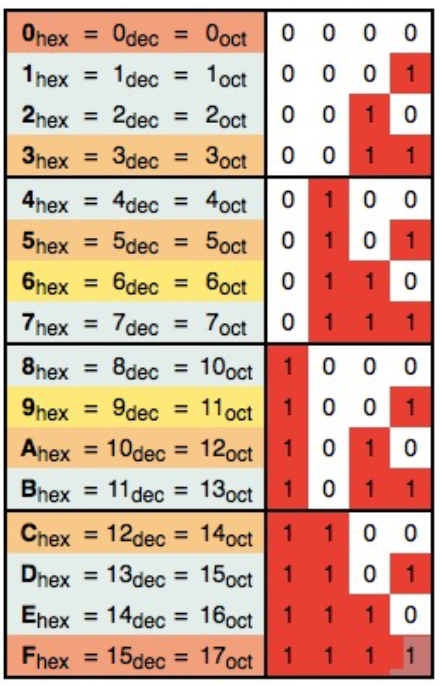
\includegraphics[width=60mm,scale=0.5]{confronto_tra_basi.png}    
\end{center}

\section{Conversione tra basi}
Svolti esercizi di conversione tra basi
\section{Operazioni aritmetiche e Overflow}
\begin{itemize}
    \item Addizzioni e sottrazioni
    \item Svolti esercizi con Overflow, bit di carry
\end{itemize}
 L'overflow di verifica quando il risultato non può essere rappresentato con il numero di bit,
 che ho a disposizione e quindi ottengo un risultato sbagliato.
\section{Operazioni con segno}
Ci sono diverse modalità per rappresentare il segno in base 2
\subsection{Modulo e segno}
La rappresentazione modulo e segno divide i bit di rappresentazione in 2, nel caso di 8 bit, 7 sono utilizzati per rappresentare il valore assoluto e il bit
più significativo (MSB - Most significant bit), quello a sinistra, rappresenta il segno, 0 positivo, 1 negativo
\begin{equation}
    1 | 0 0 0 0 1 0 0
\end{equation}
Questa rappresentazone è semplice e con n bit totali, si possono rappresentare i numeri interi nell'intervallo, ma ha alcuni problemi
\begin{itemize}
    \item Esistono 2 rappresentazioni diverse per lo 0
    \item Un bit tra tutti i bit disponibili viene speso per il segno e questo è uno spreco, riduce inoltre la capacità di rappresentazione
\end{itemize}

\subsection{Operazioni aritmetiche con MS}
Possiamo avere overflow solo quando:
\begin{itemize}
    \item si sommano due operandi con segno concorde
    \item si sottraggono due operandi con segno discorde
\end{itemize}
L'overflow si verifica quando c'è un riporto della cifra più significativa del modulo, cioè non si è nella
condizione di rappresentare il risultato ottenuto.
\subsection{Complemento a 1 (CA1)}
\'E un'altra modalità di rappresentazione dei numeri interi con segno. Come indica il nome stesso, questo metodo si basa sull'operazione di complemento

\paragraph{Complemento} è l'operazione che associa ad un bit (o ad ogni sequenza di bit) il suo opposto, cioè il valore ottento
sostituendo tutti gli 1 con 0 e uttti gli 0 con 1
\paragraph{Esecuzione} è semplice e diretta
\begin{enumerate}
    \item Se il numero da condificare è positivo lo si converte in binaro con il metodo tradizionale
    \item Sei il numero è negatio basta convertire in binario il suo modulo e quindi eseguire l'operazione di complemento sul numero appena convertito
\end{enumerate} 
\paragraph{Problema} ancora doppia rappresentazione dello 0

\subsection{Complemento a 2 (CA2)}
Anche qui il MSB è 0 se x è positivo e MSB = 1 se x è negativo
\paragraph{Esecuzione}
\begin{enumerate}
    \item Se il numero X è positivo esso rimane invariato
    \item Se il numero X è negativo
    \begin{enumerate}
        \item Si effettua il complemento a 1 (CA1) sul valore da codificare
        \item Si somma +1 al risultato ottenuto con CA1
    \end{enumerate}
\end{enumerate}
Così elimino la doppia rappresentazione dello zero. I valori negativi hanno MSB = 1.

\subsubsection{3 Metodi per il calcolo di CA2}
\begin{enumerate}
    \item Definizione di complemento alla base
    \item Per calcolare CA2 si calcola CA1 e si somma 1
    \item Regola Pratica
    \begin{enumerate}
        \item Si parte da destra, si trascrivono tutti gli 0 fino ad incontrare il primo 
        1 e si trascrive anch'esso
        \item Si complementano a 1 (0 $\to$ 1 e 1 $\to$ 0) tutti i bit restanti
    \end{enumerate}
\end{enumerate}

\title{Distinzione tra Operazione CA2 e Rappresentazone CA2}
\begin{itemize}
    \item La rappresentazione - come sono organizzati i bit
    \item Il calcolo - procedura di trasformazione
\end{itemize}

\subsection{Operazioni aritmetiche con CA2}
\subsubsection{Somma}
\begin{enumerate}
    \item Si esegue la somma su tutti i bit degli addendi, segno compreso
    \item Un eventuale riporto (carry) oltre il bit di segno (MSB) viene scartato
    \item Nel caso gli operandi siano di segno concorde occorre verificare la presenza o meno
    di overflow (il segno del risultato non  è concorde con quello dei due addendi)
\end{enumerate}
L'overflow non si presenta mai quando si sommano operandi di segno opposto.
L'overflow si presenta se:
\begin{equation}
    (+A)+(+B)=-C
\end{equation}
oppure
\begin{equation}
    (-A)+(-B) = +C    
\end{equation}
Un altro modo per vedere se c'è overflow è guardare i riporti nelle ultime 
due posizioni più significative, se sono diversi c'è overflow.
\subsubsection{Sottrazione}
La sottrazione tra 2 numeri in \textbf{CA2} viene trasformata in somma applicando la seguente Regola
\begin{equation}
    A-B=A+(-B)
\end{equation}
Tradotto in termini di CA2
\begin{equation}
    A-B=A+CA2(B)
\end{equation}
Si effettua il complemento del sottraendo
\paragraph{Overflow} Per assicurarsi della correttezza del risultato bisogna verificare l'assenza di 
Overflow:
\begin{enumerate}
    \item Non si ha overflow se gli operandi hanno segno discorde
    \item Si ha overflow se gli operandi hanno segno concorde e il segno del risultato è discorde con essi
\end{enumerate}
Gli operandi devono essere rappresentati sempre con lo stesso numero di bit, per questo motivo
in caso ci fossero meno bit si replica n volte il bit di segno (questo non altera il risultato)

\section{Operazione di Shift}
Consiste nello spostare (shit) verso destra (right) o verso sinistra (left) la posizione delle cifre di un numero, epsresso in una base qualsiasi, inserendo uno zero
nelle posizioni lasciate libere.
\begin{itemize}
    \item Left equivale a moltiplicare il numero per la base
    \item Right equivale a dividere il numero per la base
\end{itemize}
\section*{Rappresentazione Eccesso $2^n$}
Un numero X è rappresentato come segue:
\begin{equation}
    X+2^{n-1}
\end{equation}
Con n bit si rappresenta l'eccesso
\paragraph{Regola pratica} I numeri in eccesso $2^{n-1}$ si ottengono da quelli in CA2
complementando il bit più significativo
\section{Rappresentazione Eccesso 128}
Il numero è rappresentato come segue
\begin{center}
    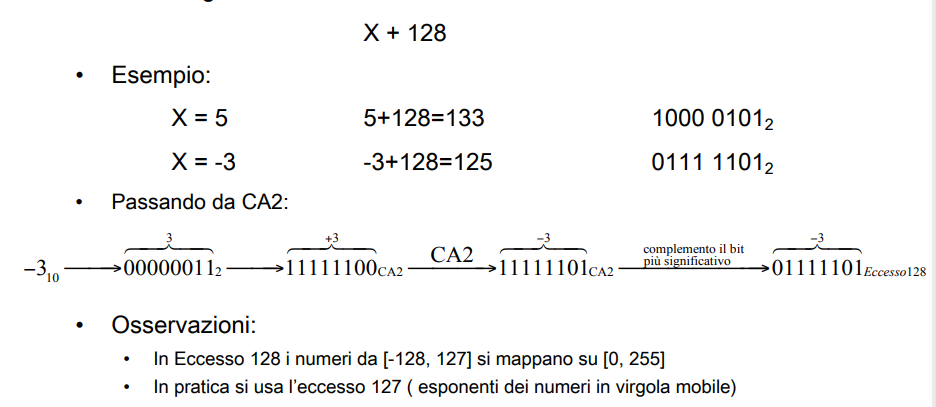
\includegraphics[width=120mm, scale=0.6]{eccesso128.png}
\end{center}

\section{Rappresentazione con la virgola}
\subsection{Virgola fissa}
\'E il metodo più semplice, scegliamo dove mettere la virgola e la fissiamo
Il problema è che in base a dove posiziono la virgola ho diverse capacità di rappresentazione della parte intera o frazionaria
\begin{itemize}
    \item Più a destra, scarsa rappresentazione intera, alta rappresentazione frazionaria
    \item Più a sinitra, scarsa rappresentazione frazionaria, alta rappresentazione intera
\end{itemize}
Questo porta rigidità

\subsection{Virgola mobile}
\begin{itemize}
    \item Usa 1 bit per rappresentare il segno s
    \item Usa altri bit per rappresentare la mantissa m
    \item Usa altri bit per codificare l'esponente e
\end{itemize}

Seguendo lo standard IEEE 754 la suddivisione è effettuata nella seguente modalità
\subsubsection{32 bit}
\begin{itemize}
    \item Segno - 1
    \item Esponente - 8
    \item Mantissa - 23
\end{itemize}
\subsubsection{64 bit}
\begin{itemize}
    \item Segno - 1
    \item Esponente - 11
    \item Mantissa - 52
\end{itemize}

\subsection{Errore assoluto ed errore relativo}
Rappresentando un numero reale n in virgola mobile si commette un errore di approssimazione,
dato che viene rappresentato un numero razionale n con un numero limitato di cifre significative
\begin{itemize}
    \item Errore assoluto
    \item Errore relativo
\end{itemize}
%Errore assoluto e relativo è Poco chiaro
\subsection{Codifiche}
Spiegazione ASCII, Unicode
%Aggiungere info

\chapter{Circuiti logici}

Nell'elettronica digitale sia ingressi che le uscite possono assumere solo i valori di sengale alto (1 per convenzione) o basso (0)

Un circuito o rete combinatoria è quel circuito

Un circuito o rete sequenziale

\section{Porte Logiche}
Le porte logiche sono i componenti elettronici che permettono di svolgere le operazioni logiche
primitive oltre che a quelle direttamente derivate.
Esse realizzano le operazioni principali dell'algebra booleana. Sono circuiti elettronici che dati dei segnali 0 e 1 in input
producono un segnale in output ottenuto effettuando una operazione booleana sugli ingressi.
Le porte logiche hanno n input e generalmente 1 output

\subsection{AND *}
Questa porta logica svolge l'operazione logica di AND tra due bit, detta anche 
\textbf{prodotto logico}.
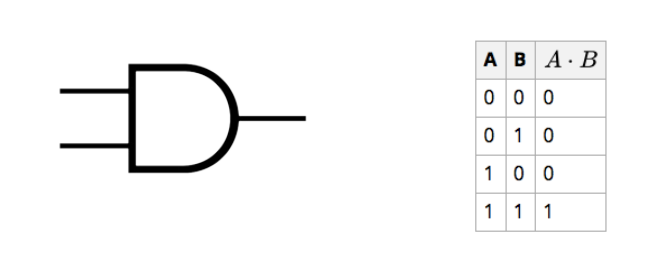
\includegraphics[width=100mm, scale=0.6]{tabella_and.png}

\subsection{OR +}
Svolge l'operazione logica di OR tra due bit, detta anche \textbf{somma logica}.
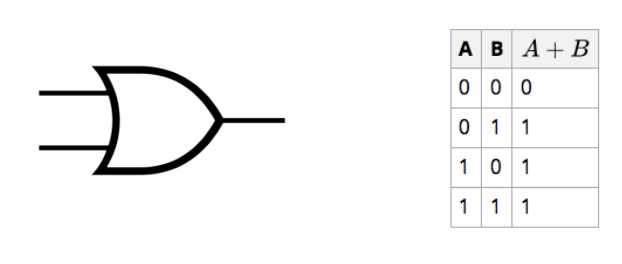
\includegraphics[width=100mm, scale=0.6]{tabella_or.png}

\subsection{NOT}
Svolge l'operazione logica di NOT su un bit, detta anche \textbf{negazione logica}.
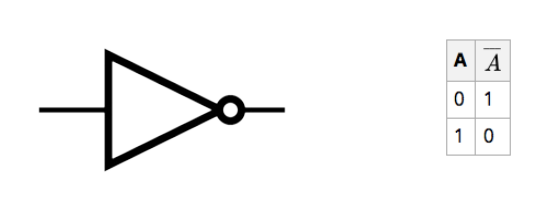
\includegraphics[width=100mm, scale=0.6]{tabella not.png}

\subsection{Port con più di due ingressi}
Ad eccezione della porta NOT, le altre porte logiche possono esistere anche ad N ingressi, queste porte
svolgono l'operazione logica associata su N bit invece che su 2.
\\ Nei circuiti si possono realizzare porte a N ingressi collegando a cascata tra loro porte a 2 ingressi.

\section{Porte logiche derivate}
Porta NAND $\to$ svolge l'operazione di NOT sul bit risultante dell'operazione di AND. 
(nega il risultato dell'and).
\\ Porta NOR $ \to $ svolge l'operazione di NOT sul bit risultante dall'operazione di OR.
(nega il risultato dell'or).
\\ Porta XOR Opera come disgiunzione esclusiva tra due input, quando i 2 bit sono uguali produce in output un 1. 
Viceversa restituisce 0.
Le porte NOR e NAND svolgono la funzione di inverter, sono definite universali
\chapter{Circuiti combinatori}
Sono circuiti dove non sono presenti memorie, l'output di un circuito combinatorio
dipende solo dall'input che stiamo dando al circuito.
\section{Decoder}
Componente elettronico caratterizzato dall'avere n ingressi e $2^n$ uscite
Solo 1 valore è attivo per ogni combinazione di input, quindi l'ingresso seleziona 
una delle uscite, l'uscita selezionata ha valore 1 tutte le altre 0.
\\ Nella foto il pallino vuoto corrisponde a 0, mentre senza pallino corrisponde a 1.
Esiste anche il suo inverso denominato encoder che riceve $2^n$ input e produce un output
di n bit.

\section{Multiplexor}
Un multiplexor, detto anche selettore, è un componente elettronico caratterizzato da
\begin{itemize}
    \item $2^n$ entrate principali
    \item n entrate di controllo (selettore)
    \item 1 uscite
\end{itemize}
Riceve n segnali in input e un solo segnale di output.
Nel caso in cui riceva 2 input (A e B) + il selector (S), il valore di output sarà A o B
in base al segnale del selettore (0 o 1, quindi True o False).
\\ Un multiplexor a 32 bit corrisponde a un array di 32 multiplexor ad 1 bit.

\subsection{Relazione importante per gli es}
La relazione tra il massimo numero di ingressi selezionabili (n) con m segnali/ingressi 
di selezioni è:
\begin{center}
    $m = \log_2 n$
    ovvero
    $n = 2^m$
\end{center}
Nel caso io abbia un multiplexor a 32 ingressi il numero di ingressi di selezione m sarà:
\begin{center}
    $2^m = 32$ ovvero $m = 5$
\end{center}


\section{Logiche a due livelli e PLA}
Possiamo creare logiche a due livelli:
\begin{itemize}
    \item Somma di prodotti: somma logica (OR) di prodotti (AND)
    \item Prodotto di somme: prodotto (AND) di somme (OR)
\end{itemize}
Esercizio tabella di verità

\textbf{Programmable Logic Array}
La somma di prodotti corrisponde ad una implementazione comunemente nota come \textbf{Programmable Logic Array}
\begin{itemize}
    \item Insieme di input
    \item I corrispondenti input complementati (mediante inverter)
    \item Una logica a due stage:
    \begin{itemize}
        \item Primo stage: un array di porte logiche AND (prodotto)
        \item Secondo stage: un array di porte logiche OR (somma)
    \end{itemize}
\end{itemize}
\begin{center}
    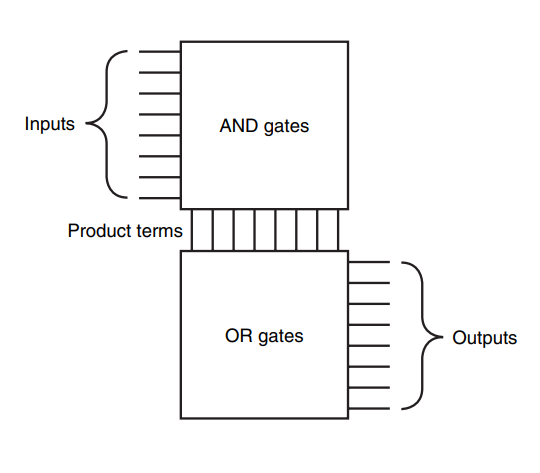
\includegraphics[width=70mm, scale=0.6]{ex_pla.png}    
\end{center}

\section{ROM (Read Only Memory)}
Circuito combinatorio in cui ad ogni ingresso (indirizzo)
corrisponde una uscita (contenuto della cella di memoria con quell'indirizzo).
\begin{itemize}
    \item Input: n bit
    \item Output: una tra le $2^n$ celle/locazioni di memoria
\end{itemize}

\paragraph{ROM vs PLA}
\begin{itemize}
    \item ROM - fully decoded VS PLA - partially decoded
    \item ROM dimensione più grande rispetto a PLA
    \item PLA più efficienti
    \item ROM possono implementare qualsiasi funzone logica
\end{itemize}

\begin{itemize}
    \item PROM (Programmable ROM) $\to$ possono essere programmate
    \item EPROM (Erasable Programmable ROM)
\end{itemize}

Normalmente il bus è di 32 bit

\section{ALU}
L'Aritmethic Logic Unit è la parte del processore che svolge le operazioni
aritmetico-logiche.
\\\'E un insieme di circuiti combinatori che implementa:
\begin{itemize}
    \item Operazioni aritmetiche, es. somma e sottrazione
    \item Operazioni logiche: es AND e OR
\end{itemize}
Blocchi per la costruzione di una ALU
\begin{itemize}
    \item AND
    \item OR
\end{itemize}
Una ALU a 32 è semplicemente l'interconnessione di 32 ALU ad 1 bit in cascata

\paragraph{Blocchi base per costruire ALU}
\begin{itemize}
    \item AND gate 
    \item OR gate
    \item Inverter
    \item Multiplexor
\end{itemize}
\subsection{Operazioni aritmetiche}
\paragraph{Addizione}
\begin{center}
    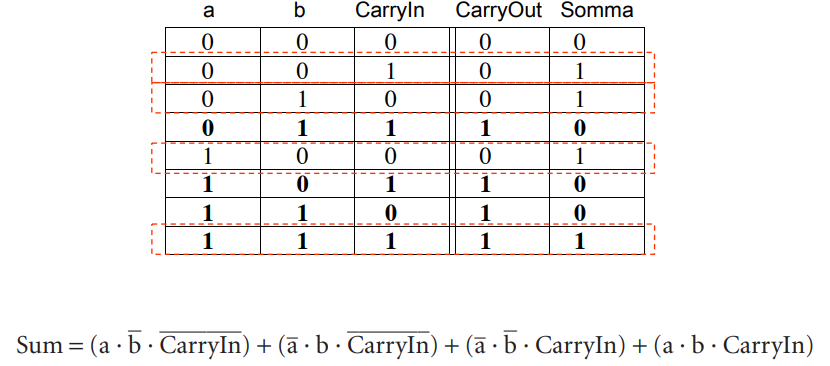
\includegraphics[width=120mm, scale=0.5]{alu_somma.png}
    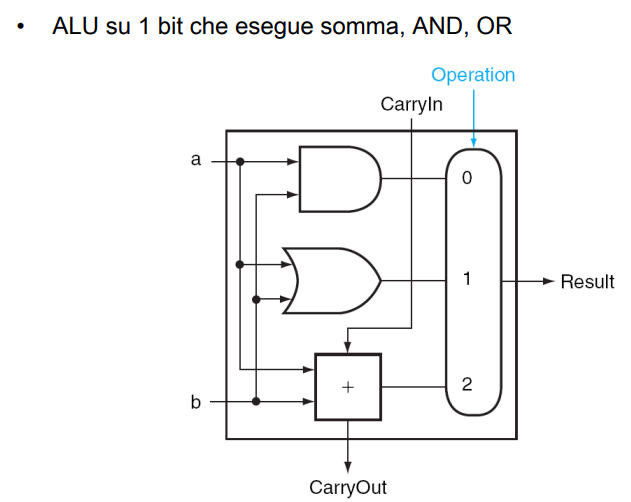
\includegraphics[width=120mm, scale=0.5]{alu_somma_circuito.png}
\end{center}
\paragraph{Sottrazione}
Negando b possiamo ottonere una sottrazione (in CA2). Per questo si aggiunge un Binvert e lo
si setta a 1 nel caso serva effettuare una sottrazione
\paragraph{NOR} si implementa con De Morgan
Connettendo 32 ALU da 1 bit otteniamo una ALU a 32 bit. La connessione si effettua collegando
il bit meno significativo con il CarryIn del bit più significativo. Questa organizzazione è
chiamata ripple carry.
\section{Operazioni di confronto - SLT e BEQ}
Le operazioni di confronto all'interno di una ALU sono BEQ (Branch-on-equal)
e SLT (set-on-less-then)
\subsection{SLT}
Risultato: 1 se a<b, 0 altrimenti.
\\ Per eseguire questa istruzione si devono poter azzerare tutti i bit dal bit-1 alcuni
bit-31 e assegnare al bit-0 il valore del risultato.
Per poter realizzare il confronto si effettua la sottrazione tra a e b.
\begin{itemize}
    \item Se $a-b < 0$ allora $a<b$ e il risultato sarà 000...01
    \item Se $a-b < 0$ allora $a>b$ e il risultato sarà 000...00
\end{itemize}
\subsection{BEQ - Branch on equal}
Per verificare l'uguaglianza di 2 elementi si fa la sottrazione fra di essi, se il risultato
è zero i due elementi sono uguali. Logicamente si fa un OR di tutte le uscite delle ALU a 1 bit
e poi si nega il risultato.
\subsection{Overflow detection}
Infine per completare la ALU è necessario inserire nell'ultima operazione un circuito
per l'overflow detection. Se all'ultima operazione è presente un bit di CarryOut si è verificato
un overflow.
\begin{center}
    Questa è il simbolo comunemente utilizzato per rappresentare la ALU. 
    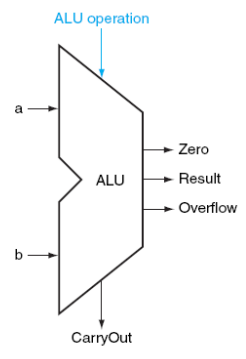
\includegraphics[width=50mm, scale=0.5]{alu_symbol.png}
\end{center}
\subsection{Carry Lookahead}
Obiettivo: anticipare i bit di CarrIn per i bit più significativi per velocizzare le operazioni
\\ Soluzione: passare tra meno porte
\\ Teniamo conto che ALU ha 3 ingressi: 2 operandi e CarryIN (per la prima ALU su 1 bit)
\begin{center}
    CarryOut0 = CarryIn1 = (b0 * CarryIn0) + (a0 * CarryIn0) + (a0 * b0)
    \\CarryOut1 = CarryIn2 = (b1 * CarryIn1) + (a1 * CarryIn1) + (a1 * b1)
\end{center}
Possiamo quindi riscrivere CarryIn2 sostituendo CarryIn1 della prima equazione
\begin{center}
    CarryIn2 = b
\end{center}

\section{Note per gli esercizi}
\subsection{Conversione da tabella a circuito}
\'E sufficiente prendere in considerazione solo le righe dove ho 1 come output, i valori 
relativi a quella riga vanno concatenati con degli AND, dato che solo se si verificano tutti
ottengo 1 come output, mentre per concatenare le righe vere fra di loro utilizzo gli OR, dato che
è sufficiente che si verifichi anche solo 1 di queste righe per poter ottenere 1 come risultato.s
\subsection{Calcolo output circuito}
Se si tratta di somme di prodotti (and concatenati da or) è sufficiente identificare un valore
che dà true dato che essendo una catenda di OR basta un solo true perchè l'espressione sia true.
Mentre è necessario controllare che siano tutti false per affermare che l'intera espressione
sia falsa.
\\Se si tratta di prodotti di somme (OR concatenati da AND) è necessario verificare che tutte le
sotto espressioni siano vere per poter affermare che l'intera espressione sia vera.
Mentre è sufficiente che una singola sotto espressione sia false per poter affermare che
l'intera espressione sia false.

\chapter{Circuiti sequenziali}
Cicuiti dove sono presenti delle memorie, per questo motivo l'output non dipende
solo dall'input che stiamo dando, ma dipende anche da valori salvati precedentemente in memoria,
questo concetto è chiamato \textbf{stato} nei blocchi logici.

\paragraph{Differenza con i circuiti combinatori} La sequenza temporale determina il valore
memorizzato nello stato.

Sintetizzando, i circuiti sequenziali sono formati da:
\begin{itemize}
    \item Elementi di memoria (di vario tipo) che memorizzano informazione
    \item Reti combinatorie che elaborano informazione
\end{itemize}

\section{Clock}
Il segnale di clock è fondamentale per le reti sequenziali caratterizzate da uno stato.
Il clock è definito come un segnale (onda quadra) con un preiodo predeterminato e costante.
\begin{center}
    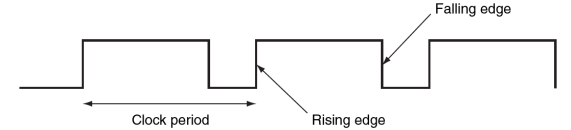
\includegraphics[width=100mm, scale=0.5]{clock_rappresentazione.png}
\end{center}
Caratterizzato da un periodo T (oppure ciclo) di clock e dalla frequenza F definita come
$\frac{1}{T}$ e misurata in Hertz.

Il periodo di Clock è abbastanza grande da assicurare la stabilità degli output di un circuito
e determina quando il contenuto di un elemento che rappresenta lo stato è aggiornato.
Sostanzialmente determina il ritmo dei calcoli e delle operazioni di memorizzazione.
\\ Con il clock il circuito diventa sincrono.
\\ La tipologia di clocking studiata è la \textbf{edge-triggered clocking}, cioè tutti i
cambiamenti avvengono sul bordo di un clock. Esistono altre tipologie di clock
utilizzate, come la \textbf{level-triggered} (utilizzata nei primi esempi), 
ma noi studieremo solo edge triggered.

\section{S-R Latch}
\textbf{S-R Latch} è un circuito composto da 2 porte NOR concatenate dove
\begin{itemize}
    \item S = Set
    \item R = Reset
\end{itemize}
\begin{center}
    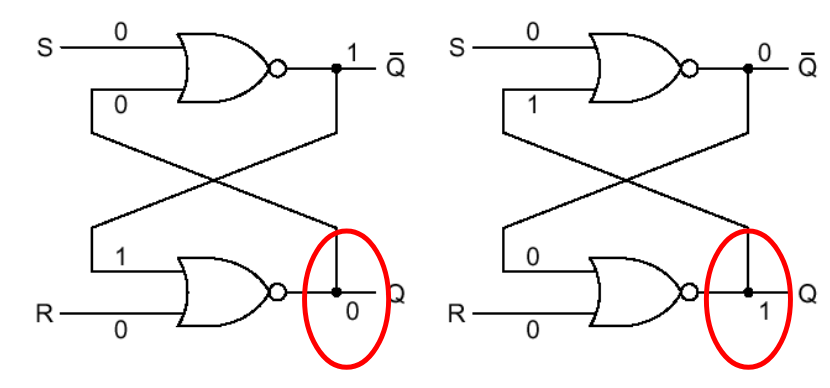
\includegraphics[width=100mm, scale=0.5]{sr_latch.png}
    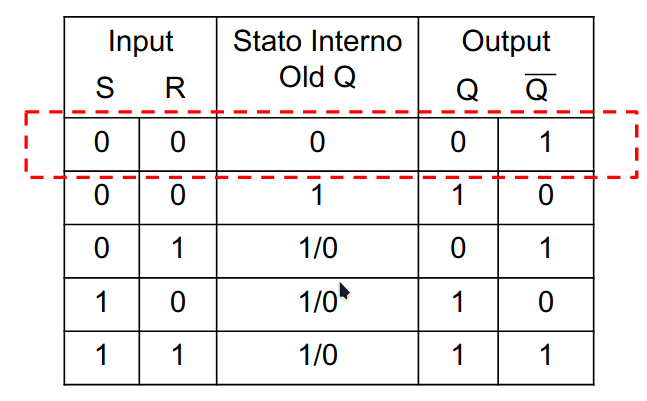
\includegraphics[width=70mm, scale=0.5]{sr_latch_tabella.png}
\end{center}

Come si può notare dalla tabella tabella di verità, il valore di set serve per
salvare un nuovo valore, quello di reset per scartare il valore salvato. Se entrambi
i valori sono a zero il valore salvato resta immutato.
\\ La combinazione set = 1 e reset = 1 va assolutamente evitata, dato che viola le
proprietà di complementarietà e può portare ad una configurazione instabile.
I valori S e R devono essere stabili e valere (1,0) o (0,1) per poter memorizzare
un valore corretto. Essi sono di solito calcolati da un circuito combinatorio.

Per evitare che vengano memorizzati i valori mentre il circuito combinatorio li sta
calcolando viene utilizzato il clock. Esso determina il tempo in cui è possibile
memoirzzare un dato.

\section{D Latch}
Caratterizzato da D = il valore da memorizzare, C = il segnale di clock, ovvero quando
il latch deve leggere e memorizzare il valore. Gli output sono sempre i valori degli
stati interni Q e il suo complementare $\neg Q$.
\begin{center}
    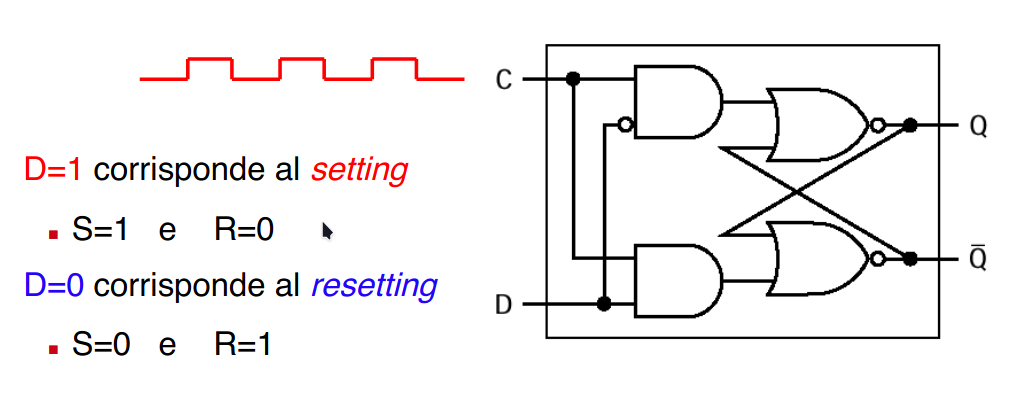
\includegraphics[width=100mm, scale=0.5]{D-latch.png}
\end{center}
\'E un Latch sincronizzato con il clock, così il latch cambia stato in momenti opportuni
Quando il clock è deasserted non viene memorizzato nessun valore, mentre quando è
asserted viene memorizzato un valore (in funzione di D).
\\Il segnale D, ottenuto come output di un circuito combinatorio deve:
\begin{itemize}
    \item Essere già stabile quando C diventa asserted
    \item Rimanere stabile per tutta la durata del livello alto di C (Setup time)
    \item Rimanere stabile per un altro periodo di tempo per evitare malfunzionamenti
\end{itemize}
Nei circuiti teorici dove il ritardo è nullo il problema non si pone, ma nei circuiti
reali il \textbf{ritardo NON è nullo}.
Gli output possono temporaneamente cambiare da valori corretti a valori errati
e ancora a valori corretti, questp fenomeno è denominato \textbf{Glitch}.
Dopo un certo intervallo, con alta probailità i segnali si stabilizzano.
\begin{center}
    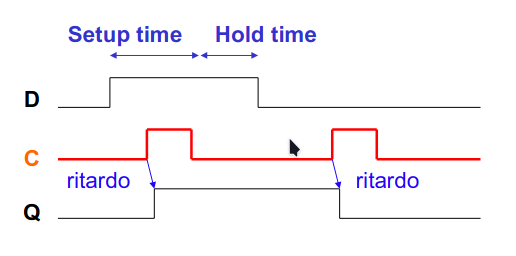
\includegraphics[width=90mm, scale=0.5]{glitch.png}
\end{center}
Per questo motivo il clock T deve essere scelto abbastanza lungo affinchè l'output
del circuito combinatorio si stabilizzi. Deve essere stabili un po' prima del periodo di apertura del
latch (setup time) e lo deve rimanere per un certo tempo (hold time).

\paragraph{Funzionamento D Latch} Quando il clock C è asserito allora il latch
è aperto e si può memorizzare il valore può essere memorizzato (il valore di output
diventa il valore di input D). Mentre quando il clock C non è asserito il latch viene detto
chiuso e il valore di output Q è il l'ultimo valore memorizzato l'ultima volta
che il latch era aperto.

\paragraph{Il D-latch è caratterizzato dal seguente comportamento}
\begin{itemize}
    \item Durante l'intervallo alto del clock il valore del segnale di ingresso D
    viene memorizzato nel latch
    \item Il valore di D si propaga quasi immediatamento all'uscita Q
    \item Anche le eventuali variazioni di D si proagano quasi immedatamente, con il
    risultato che Q può variare più volte durante l'intervallo alto del clock
    \item Solo quando il clock torna a zero Q si stabilizza
    \item Durante l'intervallo basso del clock il latch \textbf{non memorizza}
\end{itemize}

Fino ad ora abbiamo visto solo esempi con metodologia di clocking detta level-triggered,
ora vedremo la \textbf{edge-triggered}. 
\subsection{Edge-triggered clocking} In questo caso il timing avviene sul fronte di salita
(o di discesa) del clock, otteniamo così i seguenti vantaggi
\begin{itemize}
    \item La memorizzazione avviene istantaneamente
    \item L'eventuale segnale di ritorno sporco non fa in tempo ad arrivare a causa 
    dell'istantaneità della memorizzazione
\end{itemize}
Il Latch è trasparente, ma non può essere utilizzato sia come input che output
all'interno dello stesso ciclo.

\section{D Flip Flop}
Il D Flip-Flop è utilizzabile come input e output durante lo stesso ciclo di clock.
Realizzato ponendo in serie 2 D-latch: il primo viene denominato \textbf{master}
il secondo \textbf{slave}.

\begin{center}
    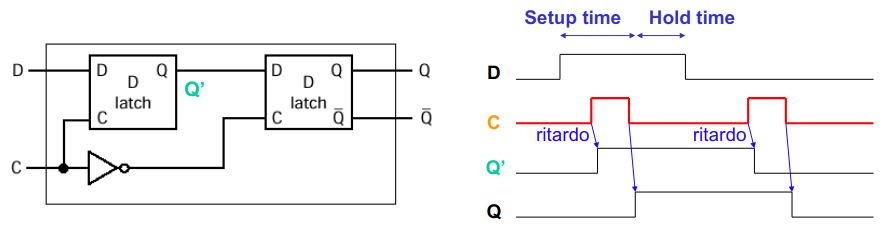
\includegraphics[width=120mm, scale=0.5]{d_flip_flop.png}
\end{center}
\begin{center}
    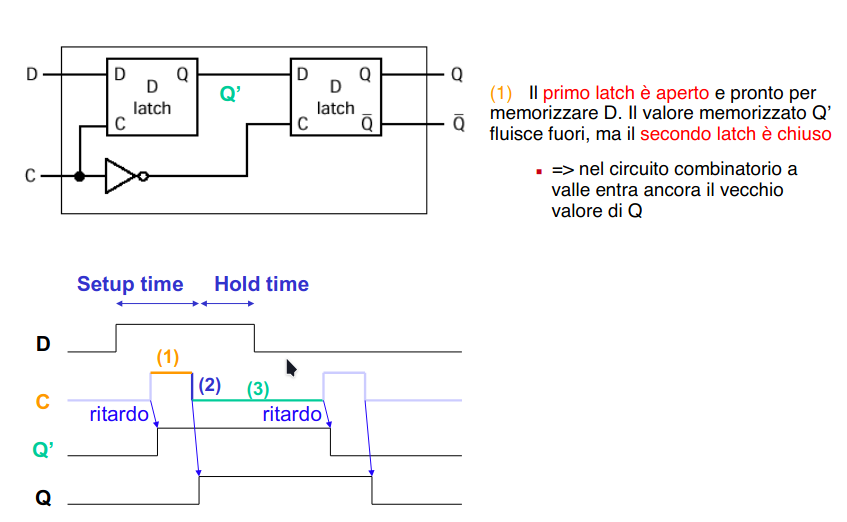
\includegraphics[width=120mm, scale=0.7]{d_flip-flop circuito.png}
\end{center}
Il Flip Flop non è trasparente, dato che il suo valore cambia solo sui on the clock
edge.

\section{Differenze tra Latch e Flip-Flop}
La principale differenza è nel momento in cui questi due circuiti operano.
\\ Il latch memorizza quando riceve un valore da memorizzare e il clock è asserito.
\\ Flip Flop invece memorizza \textbf{solo} on a clock edge.
Per questo ultimo motivo e per la possibilità di poter essere usato sia come
input che come output all'interno di un solo ciclo utilizzeremo principalmente 
flip-flop.

\section{Datapath e Register File}
Il Datapath è un insieme di unità di calcolo, come ad esempio la ALU e i registri,
necessari per l'esecuzione delle istruzioni nella CPU.
I registri sono presenti all'interno di una CPU e costituiscono una delle strutture
principali di un processore. Possono essere letti e modificati fornendo un register number
a cui accedere.
\subsection*{Implementazione}
Un registro è costituito da n flip-flop. (in MIPS ogni registro è di 1 word = 4byte = 32 bit).
I registri sono organizzati in un \textbf{Register File}.
Il Register File del MIPS ha 32 registri (32*32 = 1024 flip-flop).
Il register file permette la lettura di 2 registri e la scrittura di 1 registro.
\begin{center}
    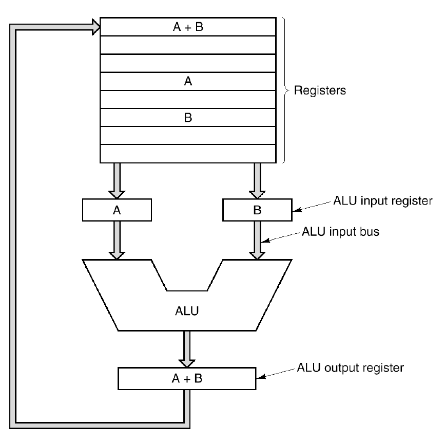
\includegraphics[width=120mm, scale=0.5]{registri.png}
\end{center}
Nel Datapath della CPU il clock non entra direttamente nei vari flip-flop,
viene messo in AND con un segnale di controllo "Write", il segnalare determina se,
in corrispondenza del fronte di discesa del clock, il valore D debba (o meno)
essere memorizzato nel registro.

\subsection*{Lettura dal Register File}
\begin{itemize}
    \item Utilizza 2 segnali che indicano i registri da leggere (Read Reg1, Read Reg2)
    \item Utilizza 2 multiplexer: ognuno con 32 ingressi e un segnale di controllo da 5 bit
    \item Il register file fornisce \textbf{sempre} in output una coppia di registri
\end{itemize}
Utilizza 3 segnali: \begin{itemize}
    \item Il registro da scrivere
    \item Il valore da scrivere
    \item Il segnale di controllo
\end{itemize}
Utilizza un decoder che decodifica il numero del registro da scrivere (Write Register)
\\ Il segnalre Write (già in AND con il clock) è in AND con l'output del decoder
\\ Se Write non è asserito nessun valore sarà scritto nel registro
\paragraph*{Alcune note}
\begin{itemize}
    \item Ogni registro può contenere valori di qualsiasi tipo purcè usino il numero
    di bit a disposizione nel registro
    \item Spetterà a chi definisce il programma in binario usare i dati
    memorizzati nei registri in modo coerente con il loro tipo
    \item Il ciclo di clock deve essere sufficientemente lungo da permettere
    al segnale di propagarsi dall'output del Register File al suo input, compreso Il
    computo della ALU.
\end{itemize}
\section{Memoria}
Oltre alle piccole memorie dei registri e file di registro esistono altri tipi di
memoria che possiamo distinguere in base a diversi parametri
\begin{enumerate}
    \item Dimensione: quantità di dati memorizzati
    \item Velocità: tempo tra richiesta e risposta
    \item Consumo: potenza assorbita
    \item Costo: costo per bit
\end{enumerate}

Non è possibile avere una memoria con tutte le caratteristiche ideali.
Possiamo però organizzare una gerarchia
\begin{itemize}
    \item Memoria piccole e più veloci (costose) sono poste ai livelli alti
    \item Memorie ampie e più lente (meno costose) sono poste ai livelli più bassi
\end{itemize}
\begin{center}
    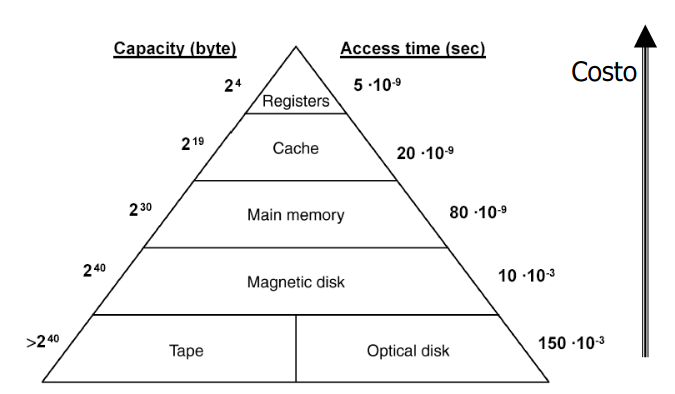
\includegraphics[width=100mm, scale=0.5]{gerarchie_memorie.png}
\end{center}

\subsection*{RAM}
La dimensione del register file è piccola, per memorizzare dati strutturati è 
necessaria una memoria più grande come la \textbf{RAM - Random Access Memory},
che è meno veloce della memoria dei registri, ma molto più capiente.
\\La RAM è un insieme di celle da 1 byte ognuna individuata da un indirizzo.
Le operazioni di lettura copiano il contenuto della cella di memoria nel registro dati,
mentre le operazioni di scrittura copiano il contenuto del Registro Dati nella cella.
\subsection*{SRAM e DRAM}
\paragraph*{Static RAM} \begin{itemize}
    \item è più veloce, tempi di accesso intorno a 0,5 - 2,5 ns
    \item vengono utilizzati dei latch per la realizzazone
\end{itemize}
\paragraph*{Dynamic RAM} \begin{itemize}
    \item Ogni bit è memorizzato tramite un condensatore
    \item tempi di accesso intorno a 50-70 ns
    \item è necessario rinfrescare il contenuto della DRAM a intervalli di tempo prefissati
\end{itemize}

\subsection*{SRAM}
\'E realizzata come matrice di latch
\begin{itemize}
    \item Larghezza o ampiezza = numero di latch pre ogni cella
    \item Altezza H = numero di celle indirizzabili
    \item Singolo indirizzo usato sia per lettura che per scrittura
    \item Non è possibile leggere e scrivere contemporaneamente
\end{itemize}

\paragraph*{Circuito SRAM}
\begin{center}
    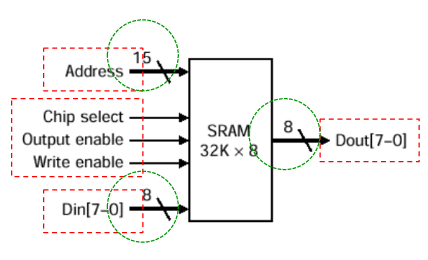
\includegraphics[width=100mm, scale=0.5]{SRAM.png}
\end{center}
\paragraph*{Spiegazione circuito}\begin{itemize}
    \item Din e Dout
    \item Address
    \item Segnali di controllo \begin{itemize}
        \item Chip select deve essere asserito per poter leggere o scrivere
        \item Output enable deve essere asserito per poter leggere
        \item Write enable deve essere asserito per poter scrivere
    \end{itemize}
\end{itemize}
\subsection*{Realizzazione SRAM}
Non è possibile utilizzare decoder e multiplexer come per i registri perchè
data la dimensione notevolmente maggiore avremmo bisogno di enormi multiplexer e decoder,
con molte porte AND, questo porterebbe all'introduzione di ritardi considerevoli agli accessi
della memoria.
\\ Per evitare multiplexer in uscita quindi: \begin{itemize}
    \item Possiamo usare una linea di bit condivisa su cui i vari elementi di memoria
    sono tutti collegati (OR)
    \item Il collegamento alla linea condivisa avviene tramite buffer a tre stati,
    che aprono o chiudono i collegamenti (se il controllo è asserito o meno)
    \item Il buffer ha due ingressi (dato e segnali di Enable) e una uscita
    \begin{itemize}
        \item l'uscita è uguale al dato (0 o 1) se Enable è asserito
        \item l'uscita viene impedita se Enable non è asserito
    \end{itemize} 
\end{itemize}
\begin{center}
    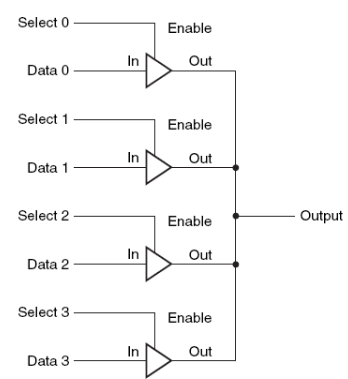
\includegraphics[width=70mm, scale=0.5]{realizzazioneSRAM.png}
\end{center}
\paragraph*{Esempio SRMA 4x2}
\begin{center}
    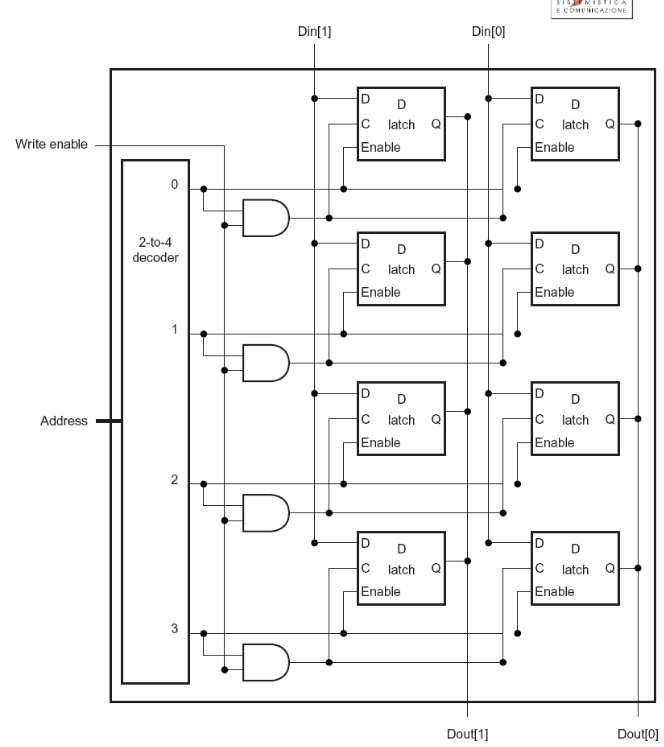
\includegraphics[width=90mm, scale=0.5]{SRAM 4x2.png}
\end{center}
I latch di una certa colonna osno collegati alla stessa linea in output (Dout[0] e Dout[1]).
\\ Nell'esempio ogni D-latch ha un segnale di Enable che abilita 
il three-state buffer interno. Il devoder serve ad abilitare in lettura e scrittura una
certa linea di memoria. Entrambi i segnali Write enable e Enable vengono abilitati
su una sola linea di memoria (2 bit).

\subsection*{SRAM a 2 livelli}
Per diminuire la complessità dei decoder è opportuno suddividere gli indirizzabili
in 2 blocchi:
\begin{enumerate}
    \item parte alta per accedere a una riga
    \item parte bassa per accedere a una specifica colonna
\end{enumerate}
Nota che celle consecutive hanno indirizzi che solitamente differiscono solo per 
la parte bassa dell'indirizzo, la parte in alto è quindi comune.
\\ Le \textbf{Synchronous SRAM e DRAM (SSRAM e SDRAM)} permettono di aumentare la banda
di trasferimento alla memoria sfruttando questa proprietà.
\\ Synchronous perchè sono sincronizzate con un segnale di clock.
\begin{itemize}
    \item è possibile specificare che vogliamo trasferire dalla memoria
    una \textbf{sequenza di celle consecutive (burst)}
    \item ogni burst è specificato da un indirizzo di partenza e da una lunghezza
    \item le celle del burst sono contenute all'interno di una stessa Riga,
    \textbf{selezionata una volta per tutte tramite decoder}
    \item La memoria fornisce una delle celle del burst a ogni ciclo di clock 
\end{itemize}
In pratica scegliendo una sequenza di celle consecutive si utilizza una volta sola
il decoder, in seguito si utilizza solo il multiplexor. Questo migliora la banda di
trasferimento, inoltre non è necessario ripresentare l'indirizzo per ottenere ogni cella
del burst.
Esempio di SRAM: 4M x 8 $\to$ servono 22 linee di indirizzo (4M = $2^{22}$)
\begin{itemize}
    \item suddiviso in 8 blocchi da 4Mb
    \item parte alta dell'indirizzo [21-10] seleziona la medesima riga di ogni blocco
    attraverso un Decoder
    \item parte bassa dell'indirizzo [9-0] seleziona singoli bit dei 1024 bit in
    output dai vari blocchi attraverso una serie di 8 Multiplexer
\end{itemize}
\begin{center}
    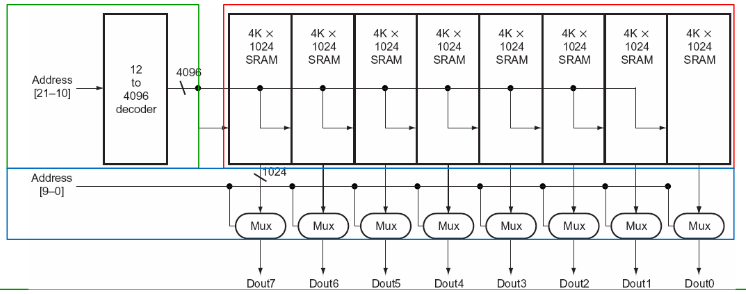
\includegraphics[width=90mm, scale=0.5]{SRAM a 2 livelli.png}
\end{center}
\paragraph{Perchè usare le DRAM}
Le DRAM sono meno costoso e più capienti rispetto alle SRAM, essendo realizzate
con un solo transistor per bit e un solo condensatore occupano meno spazio per singolo
bit, inoltre i condensatori hanno un basso costo.
Purtroppo sono più lente rispetto alle SRAM (da 5 a 10 volte più lente!). 

\paragraph{Funzionamento DRAM} 
\begin{center}
    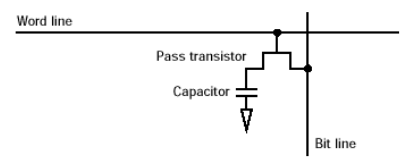
\includegraphics[width=90mm, scale=0.5]{DRAM struttura.png}
\end{center}
\begin{itemize}
    \item Il condensatore possiede una carica (0/1)
    \item Il transistor viene chiuso, trasferendo il potenziale elettrico del condensatore
    sulla Bit line (output), grazie al segnale affermato sulla Word line
    \item la specifica Word line è attivata sulla base dell'indirizzo di memoria richiesto
\end{itemize}\begin{center}
    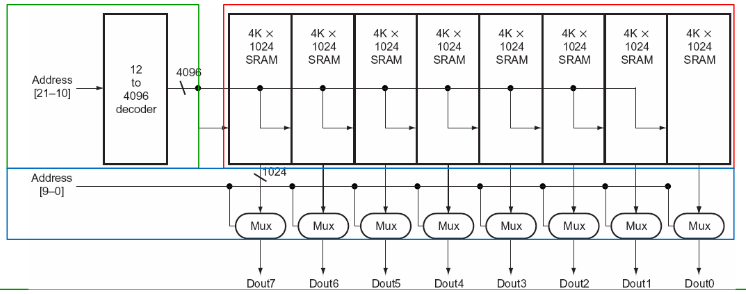
\includegraphics[width=90mm, scale=0.5]{SRAM a 2 livelli.png}
\end{center}
\paragraph{Perchè usare le DRAM}
Le DRAM sono meno costoso e più capienti rispetto alle SRAM, essendo realizzate
con un solo transistor per bit e un solo condensatore occupano meno spazio per singolo
bit, inoltre i condensatori hanno un basso costo.
Purtroppo sono più lente rispetto alle SRAM (da 5 a 10 volte più lente!). 
\section{Macchine a stati finiti}
Per la rappresentazione dei circuiti combinatori vengono utilizzate 
delle tabelle di verità, mentre per i circuiti sequenziali sono utilizzate le 
\textbf{Finite State Machine (FSM)}.
Sono composte da un set di stati e 2 funzioni 
\begin{itemize}
    \item Next state function - determina lo stato successivo partendo dallo stato corrente
    e dai valori in ingresso
    \item Output function - produce un insieme di risultati partendo dallo stato corrente
    e dai valori di ingresso
\end{itemize}
Sono sincronizzate con il clock
\begin{center}
    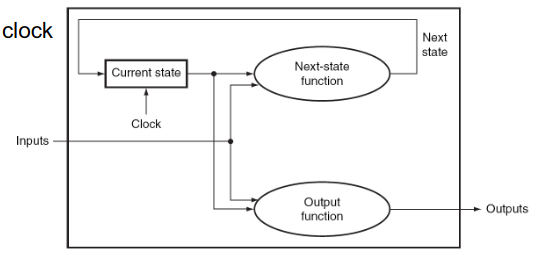
\includegraphics[width=100mm, scale=0.5]{FSM.png}
\end{center}
\paragraph*{FSM - Moore vs Mealy}
Se la macchina dipende dallo stato corrente e basta, quindi viene usata come controller
parliamo di una \textbf{FSM Moore}.
\\ Se la macchina dipende dallo stato corrente e dagli input parliamo di una FSM Mealy.
In questo corso si utilizza Moore.

\chapter{Instruction Set Architecture (ISA)}
Per analizzare l'architettura di un computer analizziamo tre aspetti
fondamentali:
\begin{itemize}
    \item Cosa fa (ISA)
    \item Come si programma (Assembly Language)
    \item Come è fatto (circuiti e Datapath)
\end{itemize}
\section{Filosofie di progetto della CPU}
Ci sono 2 principali filosofie di progetto della CPU
\begin{itemize}
    \item RISC (Reduced Instruction Set Computing)
    \item CISC (Complex Instruction Set Computing)
\end{itemize}
\subsection{RISC}
\begin{itemize}
    \item Poche istruzioni semplici
    \item Struttura circuitamente semplice
    \item Esecuzione veloce di una singola operazione
    \item Occorrono più istruzioni per fare cose anche semplici
\end{itemize}
Ottimi esempi di questa tipologia di architettura sono MIPS, ARM e PowerPC.
\paragraph{Implementazioni} MIPS è stata utilizzata per i processori del Nintendo64,
mentre PowerPC per quanto riguarda PlayStation , Xbox 360, Nintendo Wii e GameCube.

\subsection{CISC}
\begin{itemize}
    \item Istruzioni complesse
    \item Struttura circuitalmente complicata
    \item Esecuzione più lenta di una singola istruzione
    \item Occorrono meno istruzioni
\end{itemize}
Un esempio diffusissimo è Intel x86 e tutti i derivati.

\section{Istruzioni MIPS}
Noi utilizzeremo MIPS attraverso QTSPIM.
Essendo RISC è semplice, uniforme e più semplice da capire. 
Utilizza 32 registri di 32 bit e istruzioni di 32 bit.

Ogni istruzione ha un formato diverso, quindi raggruppa di 32 bit in modo diverso.
In MIPS le istruzioni sono divise in tre formati
\begin{itemize}
    \item R-type - Istruzioni relative ai registri
    \item I-type - Istruzioni immediate (costanti passate direttamente nel codice dell'operazione)
    \item J-type
\end{itemize}

\subsection{R-Type}
Sono le istruzioni che operano sui registri
Formato istruzione.
\begin{center}
    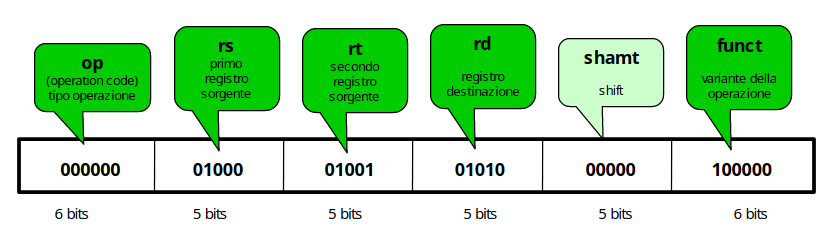
\includegraphics[width=100mm, scale=0.5]{R-type format.png}
\end{center}
\paragraph*{OpCode} In questo caso l'opcode dice che è di tipo R dato che le R-type Instruction
hanno tutte OpCode 000000. Per identificare l'istruzione è necessario controllare il 
campo funct. Per gli altri tipi di istruzione non esiste.
\subsubsection*{Shift left)}
\begin{center}
    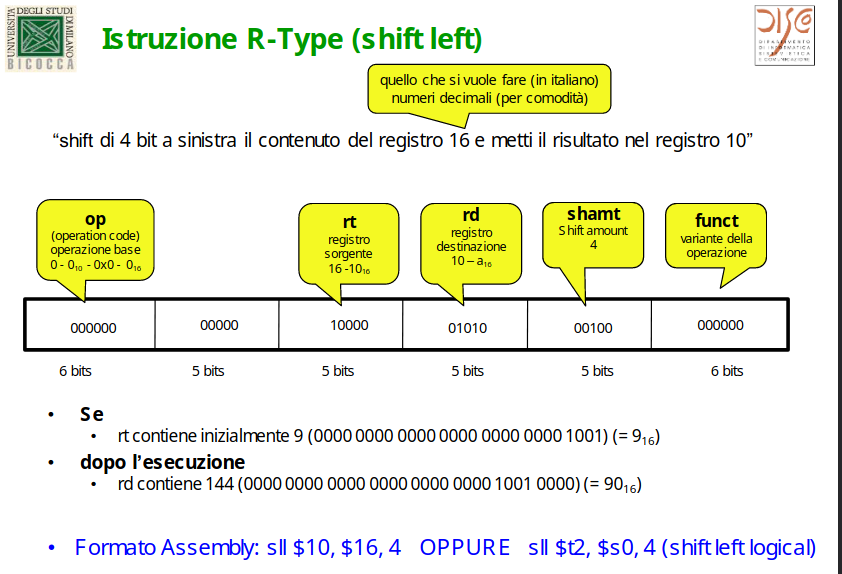
\includegraphics[width=100mm, scale=0.5]{Shift left.png}
\end{center}

\subsection{I-type}
Istruzoni per la somma di valori ricorrenti (costanti), in questo caso la costante viene direttamente
passata nel codice dell'operazione, riservando 16 bit per il valore (campo passato in complemento a 2).
Vengono chiamate I-type perchè si tratta di operazioni immediate.
Il valore è considerato come un intero con segno ($2^{15}$ valori rappresentabili)
Il formato è il seguente:
\begin{center}
    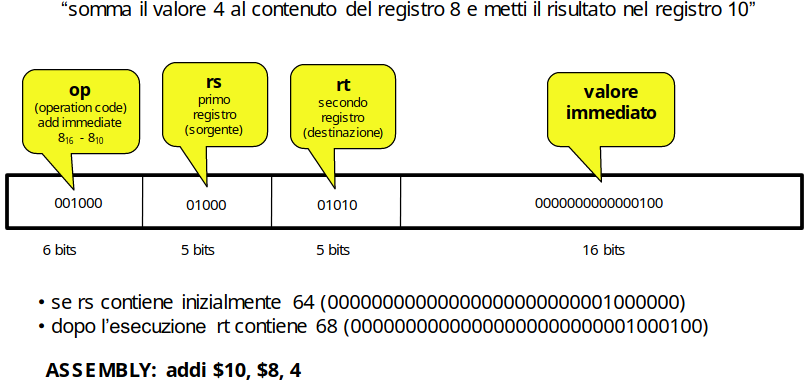
\includegraphics[width=100mm, scale=0.5]{I-type format.png}
\end{center}
Chiaramente le stringhe di bit sono poco leggibili, per questo esiste assembly.
Scrivo delle parole e attraverso un assembler lo trasformo in linguaggio macchina, traduco
quindi il codice sorgente in eseguibile.
\paragraph{Indirizzamento della memoria} Nota utile per la spiegazione della prossime istruzioni
\begin{center}
    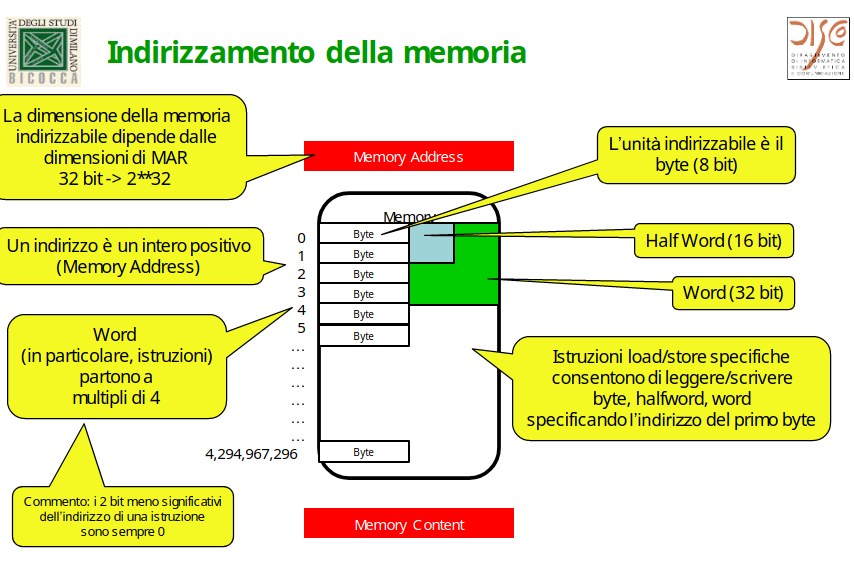
\includegraphics[width=100mm, scale=0.5]{assembly indirizzamento memoria.png}
\end{center}

\subsubsection*{Load and Store}
Istruzione per prelevare un valore dalla memoria RAM e salvarlo in un registro della CPU.
Istruzione composta da:
\begin{itemize}
    \item opcode
    \item Registro di destinazione
    \item Indirizzo di memoria il cui contenuto viene copiato nel registro destinazione
\end{itemize}
\paragraph{Problema} La memoria è grande, in MIPS ho $2^{32}$ locazioni, 
per specificare un indirizzo occorrone 32 bit, ma non ci stanno in una istruzione di appunto
32 bit. 
\paragraph*{Soluzione} Usare il formato I-type (opcode, 2 registri, 1 immediato), dove un
registro è la destinazione, un registro contiene un indirizzo base e il valore immediato
è interpretato come l'offset (spiazzamento) rispetto all'indirizzo base.
L'indirizzo a cui accedere è calcolato quindi come (base + offset).
\paragraph*{Esempio Load Word MIPS}
\begin{center}
    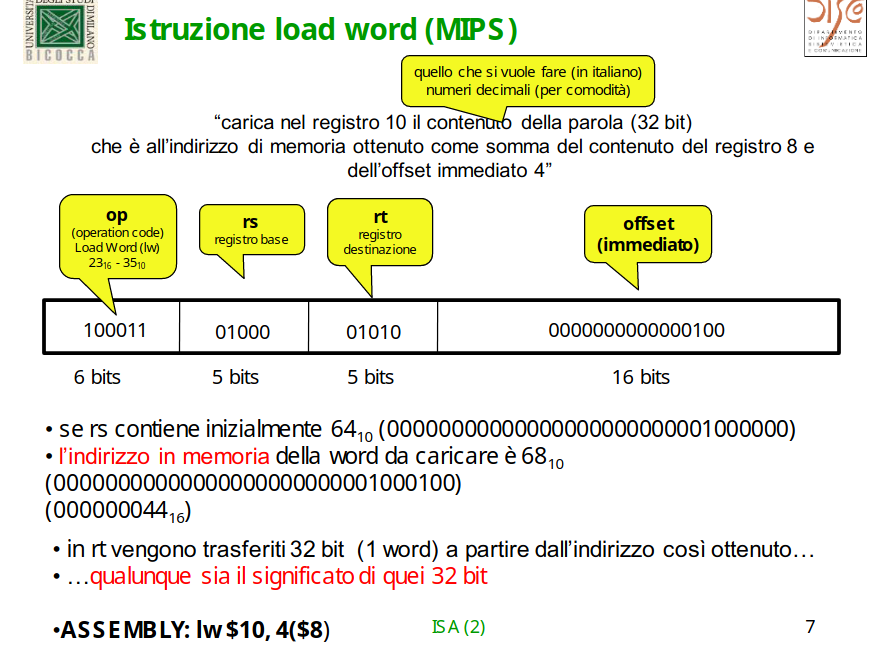
\includegraphics[width=100mm, scale=0.5]{load and store.png}
\end{center}
\paragraph*{Rappresentazione grafica esecuzione Load Word}
\begin{center}
    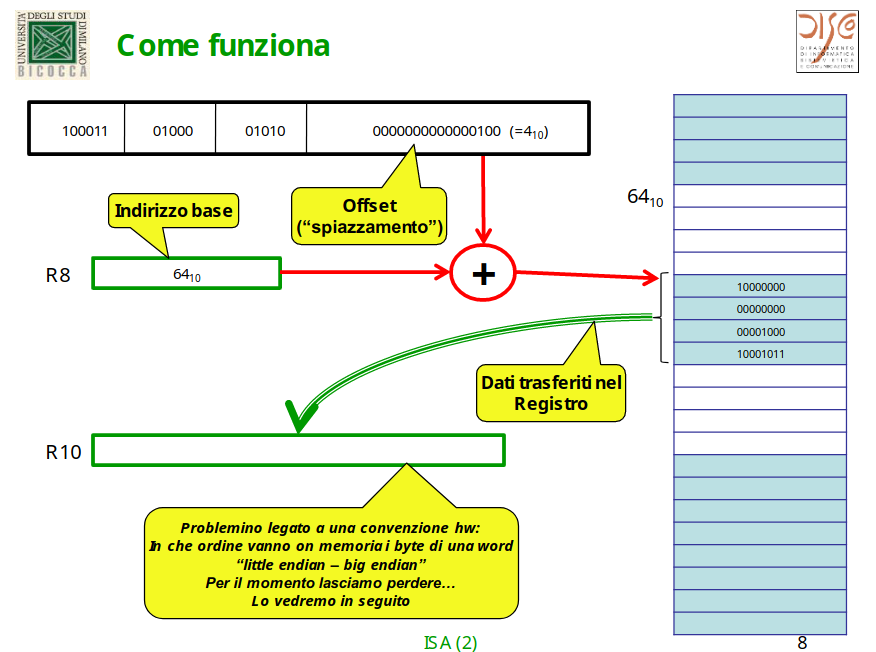
\includegraphics[width=100mm, scale=0.5]{funzionamento ld.png}
\end{center}
Il problema del little endian - big endian è un problema di convenzione,
alcuni calcolatori considerano i bit ricevuti in memoria dal più significativo
al meno significativo, altri il contrario, più avanti si affronterà la soluzione
a questo problema.

\subsubsection*{Store word}
In questo caso viene memorizzato il contenuto di un registro del processore direttamente
in memoria RAM. Viene sempre utilizzata la tecnica della rappresentazione di un indirizzo di
memoria come "indirizzo base + offset"
\begin{center}
    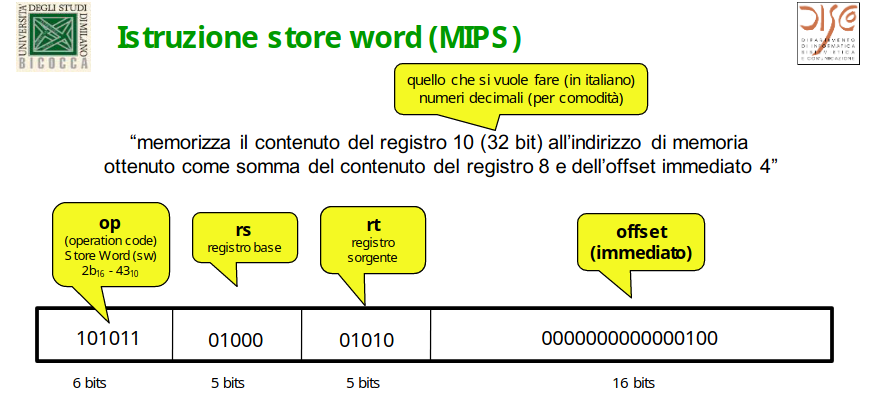
\includegraphics[width=100mm, scale=0.5]{store word.png}
\end{center}

\subsubsection*{Branch on not equal}
Sempre istruzione I-Type, mi permette di saltare a Branch Address se il contenuto
del primo registro è diverso dal contenuto del secondo.
\begin{center}
    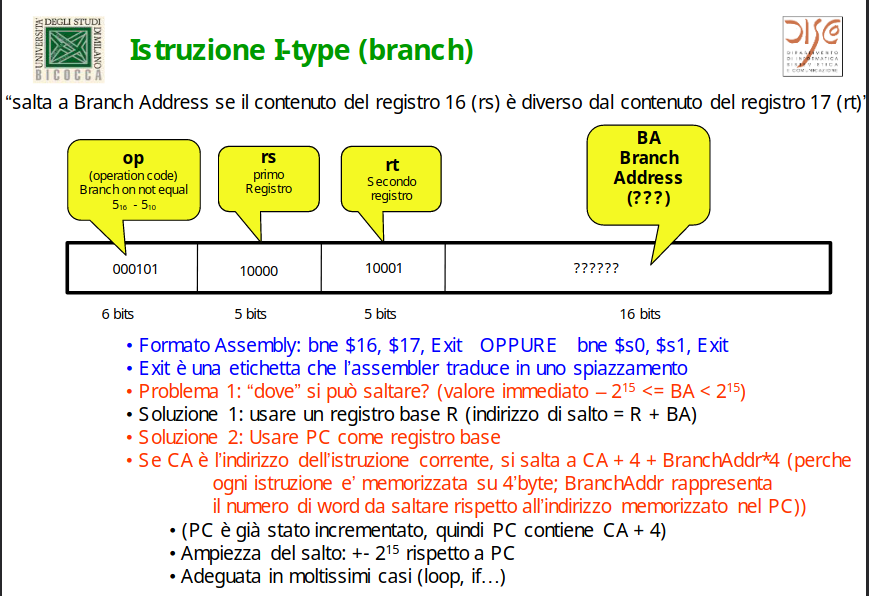
\includegraphics[width=100mm, scale=0.5]{branch.png}
\end{center}


\subsection{J-type}
Istruzioni caratterizzate dal fatto che ci sia un salto (jump) a un determinato
indirizzo.

\subsubsection*{Jump}
L'istruzione Jump mi permette di saltare a una specifica istruzione tramite indirizzo.
\begin{center}
    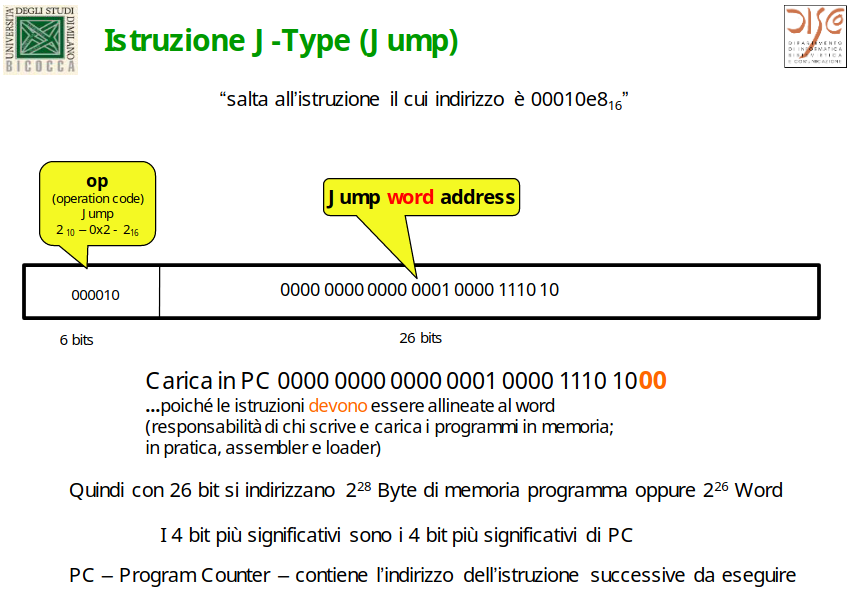
\includegraphics[width=100mm, scale=0.5]{jump.png}
\end{center}

\section{Procedure e convenzioni registri}
Questa sezione tratterà il passaggio di parametri attraverso registri per esempio
per il controllo del flusso del programma.

\subsection*{Istruzione jal - jump and link}
\paragraph*{Sintassi} jal "IndirizzoProcedura".
\\ Questa istruzione salta a una procedura indicata nella stessa e contemporaneamente
crea un collegamento a dove deve ritornare per continuare l'esecuzione del chiamante.
Salva nel registra \$ra, return adress situato nel registro 31, l'indirizzo a cui tornare
dopo l'esecuzione della procedura.
\'E l'indirizzo successivo a quello dell'istruzione jal, cioè l'indirizzo in cui si trova
la jal + 4. Tale indirizzo si trova nel regisro PC (Program Counter). 

\subsection*{jr - jump register}
\paragraph*{Sintassi} jr "registro".
\\ Salta all'indirizzo contenuto in un registro. \'E una istruzione di uso generale
che consente di saltare a qualsiasi locazione di memoria.
\paragraph*{Utilizzo tipico di jr} jr \$ra. In questo modo realizzo il ritorno da procedura,
saltando all'indirizzo precedentemente salvato da jal.

\subsection{Passaggio parametri - convenzioni base registri}
Riporto per chiarezza uno screenshot di QTSPIM per chiarire la denominazioni dei registri
della CPU.
\begin{center}
    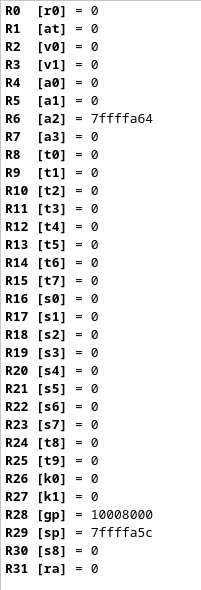
\includegraphics[width=50mm, scale=0.5]{QTSPIM Reg.png}
\end{center}
\begin{itemize}
    \item \$r0 (0): contiene sempre il valore 0
    \item \$at (1), \$k0 (26) e \$k1 (27): sono riservati per l'assembler e il sistema operativo
    \item \$a0 - \$a3 (4-7): registri argomento per il passaggio dei parametri
    \item \$v0, \$v1 (2,3): registri valore per la restituzione dei risultati
    \item \$t0 - \$t9 (8-15, 24, 25): chiamati \textbf{caller-saved register} sono utilizzati per memorizzare quantità temporanee
    che non serve che vengano preservate tra le calls
    \item \$s0 - \$s7 (16-23): chiamati \textbf{callee-saved register} utilizzati per contenere valori per un tempo lungo, valori
    che devono essere preservati attraverso le calls.
    \item \$gp (28): puntatore globale che punta a metà di un blocco di memoria da 64K 
    \item \$sp (29): stack pointer, punta l'ultima posizione sullo stack
    \item \$fp (30): frame pointer
    \item \$ra (31): return address from a procedure call (l'istruzione jal scrive in questo registro)
\end{itemize}
\subsection{Convenzioni sui registri t e s}
\paragraph{I registri \$t (temporary) non sono salvati dalla procedura} 
\begin{itemize}
    \item il chiamante non si può aspettare di trovare immutati i contenuti dei registri 
    \$t dopo una chiamata a procedura
    \item I contenuti dei registri \$t devono essere salvati dal chiamante prima della chiamata
    a procedura
\end{itemize}

\paragraph{I registri \$s (saved) sono salvati dalla proceudra}
\begin{itemize}
    \item Il chiamante ha il diritto di aspettarsi che i contenuti dei registri \$s siano
    immutati dopo una chiamta a procedura
    \item Se la procedura usa i registri \$ s deve salvarne il contenuto all'inizio e
    ripristinarlo prima del ritorno
\end{itemize}
Il contenuto dei registri \$s viene salvato sullo \textbf{stack}. 
\paragraph{Procedura foglia e non foglia}
Una procedura foglia non chiama altre procedura, mentre una procedura NON foglia chiama altre
procedure.
Se una procedura chiama un'altra procedura è necessario salvare il contenuto dei registri \$ ra
e \$s sullo stack.
\\ Per convenzione i registri \$a0 -\$a3 sono utilizzati per il passagio dei parametri.
\\ Mentre gli indirizzi \$v0 - \$v1 sono utilizzati per la restituzione dei risultati.
\\ Dal punto di vista hardware sono registri come tutti gli altri, ma il loro utilizzo
per il passaggio di parametri e risultati è una convenzione programmativa che deve 
essere rispettata per consentire di scrivere procedure che possono essere scritte
senza bisogno di sapere come è fatto il programma che le chiama e possono essere chiamate
senza bisogno di sapere come sono fatte "dentro".
\paragraph*{NB un parametro può essere un dato o un indirizzo!}
\paragraph*{I 6 passi di una procedura}
\begin{itemize}
    \item Setting dei parametri in un luogo accessibile alla procedura
    \item Trasferire il controllo alla procedura e salvare l'indirizzo
    dell'istruzione dove tornare dopo la chiamata della procedura (usare jal)
    \item Acquisire risorse per l'esecuzione della procedura
    \item Eseguire il compito richiesto
    \item Mettere il risultato in un luogo accessibile al chiamante
    \item Restituire il controllo al punto di partenza (usare l'istruzione jr)
\end{itemize}

% Rivedere esempi PDF procedure

\chapter{ASM - Catena Programmativa + Linguaggio Assembly}
\section{Linguaggio Assembler - Vantaggi e Svantaggi}
\paragraph*{Vantaggi} La dipendeza dall'architettura del calcolatore porta a numerosi vantaggi
\begin{itemize}
    \item Più efficienza
    \item Programmi potenzialmente più compatti
    \item Massimo sfruttamento delle potenzialità dell'hardware sottostante
    \item Molto importante per programmare controller di processi e macchinari o per 
    apparati limitati (embedded)
\end{itemize}
\paragraph*{Svantaggi}
\begin{itemize}
    \item meno espressività (strutture di controllo limitate)
    \item Necessario conoscere i dettagli dell'architettura
    \item Mancaza di portabilità su architetture diverse
    \item Difficoltà di comprensione
    \item Lunghezza maggiore dei programmi
\end{itemize}

\section{Compiler, Assembler, Linker}
\begin{center}
    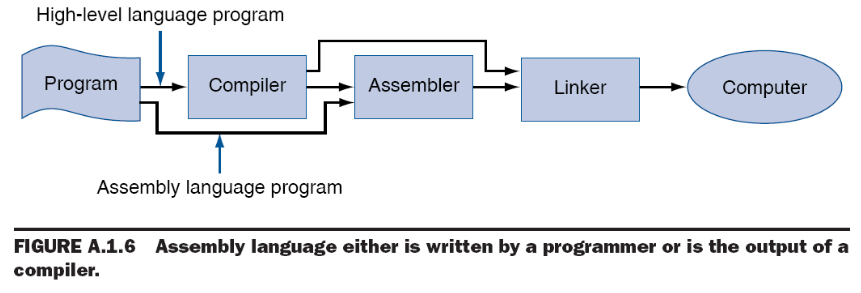
\includegraphics[width=100mm, scale=0.5]{compiler_assebler_linker.png}    
\end{center}
\begin{center}
    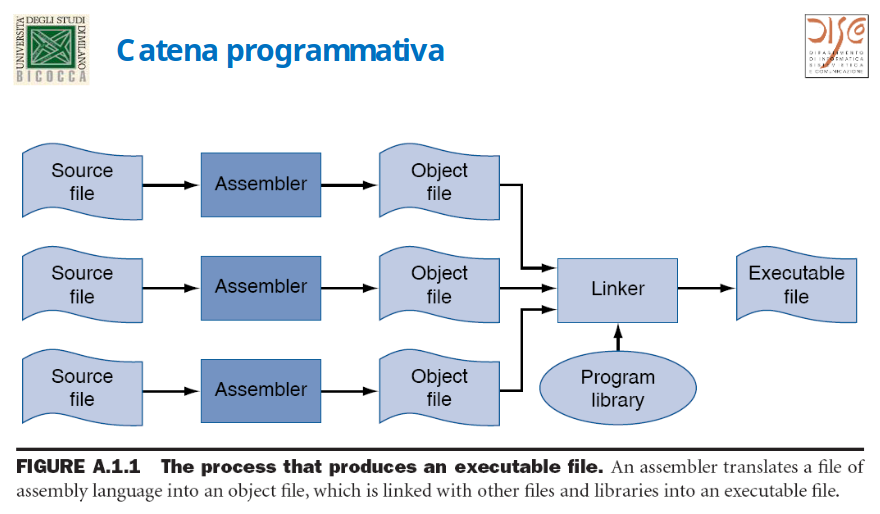
\includegraphics[width=100mm, scale=0.5]{catena programmativa.png}
\end{center}

\paragraph*{Debugger}
Consente di eseguire il programma in modo controllato per la ricerca di un bug.
Programma eseguito passo per passo e ispezione del valore di variabili ed espressioni.
Possibilità di interrompere in punti predefiniti (breakpoint) e di interruzione in caso di modificati
del valore di determinate variabili (watchpoint). Visualizzazione degli indirizzi di memoria
delle variabili o delle istruzioni.

\subsection{Compilatore}
Un programma ad alto livello viene tradotto nel linguaggio assembly utilizzando un
apposito programma detto compilatore. Dopo la fase di compilazione, il programma scritto
in linguaggio assembly viene tradotto in linguaggio macchina da un apposito programma \textbf{l'assemblatore}.
\\ Spesso con il termine compilazione si indica l'intero processo di traduzione da linguaggio
ad alto livello a linguaggio macchina (essendo l'assemblatore spesso integrato con il compilatore).

\subsection{Assembler}
\begin{itemize}
    \item Converte un programma assembler (file sorgente) in linguaggio macchina (file oggetto).
    \item Gestisce le etichette
    \item Gestisce pseudoistruzioni
    \item Gestisce numeri in base diverse
\end{itemize}

\subsection{Il processo di assemblaggio}
L'assemblaggio è un procedimento sequenziali che esamina, riga per riga il codice sorgente
Assembly, traducendo ciascuna riga in un'istruzione del linguaggio macchina.
Viene applicato modulo per modulo al programma costituisce per ogni modulo la tabella dei 
simboli del modulo.
2 passi importanti \begin{itemize}
    \item Traduce i codici mnemonici (simbolici) delle istruzioni nei corrispondenti
    codici binari
    \item Traduce i riferimenti simbolici (variabili, registri, etichete di salt, parametri)
    nei corrispondenti indirizzi numerici.
\end{itemize}
Poichè le etichette di salto generano il problema dei riferimenti in avanti (ossia,
riferimenti ad etichette successive o contenute in altri file), l'assemblatore deve leggere
il programma sorgente due volte.
\\ Ogni lettura del programma sorgente è chiamata passo e l'assemblatore è chiamato traduttore
a 2 passi.
\\ Ogni modulo assemblato di default parte dall'indirizzo 0
\paragraph*{Tabella dei simboli} Contiene i riferimenti simbolici presenti nel modulo
da tradurre e al termine del primo passo, conterrà gli indirizzi numerici di
di tutti i simboli, tranne quelli esterni al modulo in esame.
Per le etichette associate a direttive dell'assemblatore che definiscono costanti
simboliche viene creata la coppia "etichetta, valore" e in ogni istruzione che
fa riferimento al simbolo viene sostitito il valore.
\\ Discorso simile per le etichette che definiscono variabili (spazio di memoria +
eventuale inizializzazione). In questo caso l'assemblatore riserva spazio, eventualmente
inizializza la zona di memoria e crea nella tabella la coppia "etichetta, indirizzo".
In ogni istruzione fa riferimento al simbolo (all'etichetta), il simbolo viene
sostituito con l'indirizzo.
Nelle etichette presenti nelle istruzioni di salto, l'assemblatore deve generare un
riferimento all'indirizzo dell'istruzione destinazione di salto.
\paragraph*{Osservazioni} Le etichette esterne (global) al modulo possono essere usate
da moduli esterni, mentre le etichette interne (local) sono visibili solo all'interno 
di un modulo.
\\ Le etichette esterne a un modulo rimangono non risolte, ma l'assembler non è disturbato
da questo aspetto, dato che esse saranno risolte poi dal \textbf{linker}.

\subsection{Linker (Link editor)}
Dopo che l'assembler ha tradotto il sorgente in vari moduli non resta che integrarli
fra di loro e creare una singola unità eseguibile, a questo ci pensa il \textbf{linker}.
Il linker principlamente effettua le seguenti operazioni:\begin{itemize}
    \item Inserisce in memoria in modo simbolico il codice e i moduli dati
    \item Determina gli indirizzi dei dati e delle etichete che compaiono nelle istruzioni
    \item Corregge i riferimenti interni ed esterni e risolve i riferimenti in sospeso (a etichette esterne)
    \item Genera il file eseguibile
\end{itemize}
Quindi ora abbiamo il file il linguaggio macchina pronto per essere eseguito.
\begin{center}
    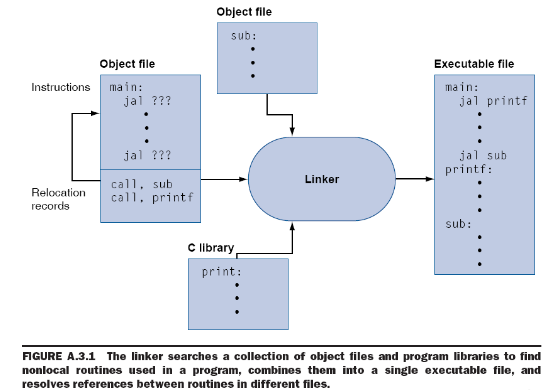
\includegraphics[width=100mm, scale=0.5]{linker.png}
\end{center}
\subsection{Loader}
Quando eseguiamo un programma interviene il \textbf{loader}.
\'E la parte che si occupa del caricamento del programma e delle relative librerie in memoria,
prepara inoltre l'esecuzione da parte del sistema operativo.
Nel dettaglio: \begin{itemize}
    \item Viene letta l'intestazione del file eseguibile per determinare la lunghezza
    del segmento di testo (cioè delle istruzioni) e del segmento dati (cioè le variabili)
    \item Viene creato uno spazio di indirizzamento sufficiente a contenere testo e dati
    \item Vengono copiate delle istruzioni e dati dal file esegubile in memoria
    \item Vengono copiati nello stack eventuali parametri passati al programma principale
    \item Inizializzati i registri e impostato lo stack pointer affinchè punti alla prima
    locazione libera
    \item Salto a una procedura di startup la quale copia i parametri nei registri argomento
    e chiama la procedura principale del programma
    \item Quando la procedura principale restituisce il controllo, la procedura di
    startup termina il programma con una chiamata alla funzione di sistema exit
\end{itemize}

L'assemblatore riceve delle ridettive in fase di assemblaggio, queste non corrispondono
a istruzioni macchina e servono per: \begin{itemize}
    \item associare etichette simboliche a indirizzi
    \item allocare spazio di memoria per le variabili
    \item decidere in quali zone di memoria allocare istruzioni e dati
\end{itemize}

\subsection{Pseudoistruzioni}
Istruzione assemblu che non ha una corrispondente istruzione macchina, viene tradotta
dall'assembler in una sequenza di istruzioni.

\section{Uso dello stack}
\begin{center}
    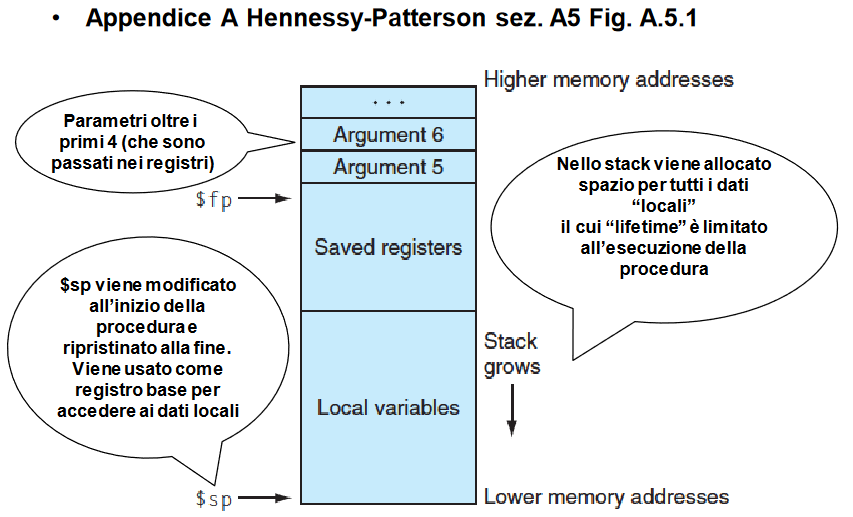
\includegraphics[width=100mm, scale=0.5]{uso dello stack.png}
\end{center}
Lo stack è l'area di memoria dove vegono salvati gli indirizzi delle procedure che devono
essere richiamate.
Cosa fa la procedura? Alloca spazio nello stack
\begin{itemize}
    \item Decrementa \$sp per lasciare in stack lo spazio necessario al salvataggio (1 word
    per ciascun registro da salvare)
    \item Salva \$ra
    \item Salva eventuali altri registri usando \$sp come registro base
    \item Ripristina i registri
    \item Incrementa \$sp per riportarlo alla situazione inizializzazione
    \item Jr \$ra (ritorno alla procedura)
\end{itemize}

I registri che interagiscono con lo stack sono: \begin{itemize}
    \item \$sp che punta alla prima parola del frame
    \item \$fp che punta all'ultima parola del frame
\end{itemize}
Un frame di solito è multiplo della parola doppia (8 byte).
\\Esempio: un frame di 32 byte
\begin{lstlisting}
    addi $sp, $sp, -32 # frame di stack di 32 byte
    addi $fp, $sp, 28 # imposta il frame pointer
    sw $ra, 0($fp) # salva l'indirizzo di ritorno 
                   # come primo word nel frame sullo stack
\end{lstlisting}

\subsection{Operazioni procedura chiamante}
Prima di chiamare una procedura, la procedura chiamante deve eseguire i seguenti passi
 al fine di non avere perdita di informazione:
\begin{itemize}
    \item Impostare gli argomenti da passare alla procedura in \$a0 - \$a3, eventuali
    altri argomenti sono nella memoria o nello stack
    \item Salvare eventualmente i registri \$a0 - \$a3 e \$t0 - \$t0 in quanto la procedura
    chiamata può usare liberamente questi registri
    \item Infine chiamare la procedura tramite istruzione \textit{jal "nome procedura"}
\end{itemize}

\subsection{Operazioni procedura chiamata}
La procedura chiamata chiamata deve eseguire i seguenti passi \textbf{appena viene chiamata}
\begin{itemize}
    \item Allocare il suo stack frame (\$sp = \$sp - dimensione frame procedura)
    \item Salvare i valori disponibili nei registri \$s0 - \$s7, \$fp, \$ra se intende
    usare tali registri per la sua esecuzione, se per esempio la procedura non chiama
    un'altra procedura non è necessario salvare il registra \$ra
    \item Settare il frame pointer (che indica l'indirizzo dell'ultima parola del frame)
    \$fp = \$sp - dimensione frame procedura + 4
\end{itemize}

Quando \textbf{ha finito la sua esecuzione} deve eseguire i seguenti passaggi
\begin{itemize}
    \item Mettere il valore di ritorno nei registri \$v0, \$v1
    \item Ripristinare i valori dei registri salvati sullo stack (\$s0 - \$s7. \$fp, \$ra)
    \item Liberare lo spazio sullo stack: \$sp = \$sp + dimensione frame procedura
    \item Eseguire l'istruzione \textit{jt \$ra}
\end{itemize}

\section{Syscall}
In un sistema reale esiste il Sistema Operativo che è un insieme di programmi che: \begin{itemize}
    \item stanno in un'area (protetta) di memoria
    \item svolgono funzioni di utilità generale (in particolare I/O) richiamabili dai
    programmi utente
\end{itemize}
Qui tratteremo i meccanismi base di chiamata al SO. Il simulatore MIPS fornisce alcune
funzioni elementare che simulano alcune funzionalità base del SO, richiamabili attraverso
il meccanismo di \textbf{syscall}, concettualmente analogo a una chiamata a procedura.
\\ Per effettuare una syscall è sufficiente inserire nel registro \$v0 il codice della syscall
e nei registri \$a0-\$a3 gli argomenti.

\paragraph{Syscall essenziali}
\begin{itemize}
    \item exit2 codice 17: terminazione del programma
    \item read\_int
    \item print\_int codice 1 (parametro passato per valore)
    \item read\_string
    \item print\_string (parametro passato per indirizzo)
\end{itemize}

\begin{center}
    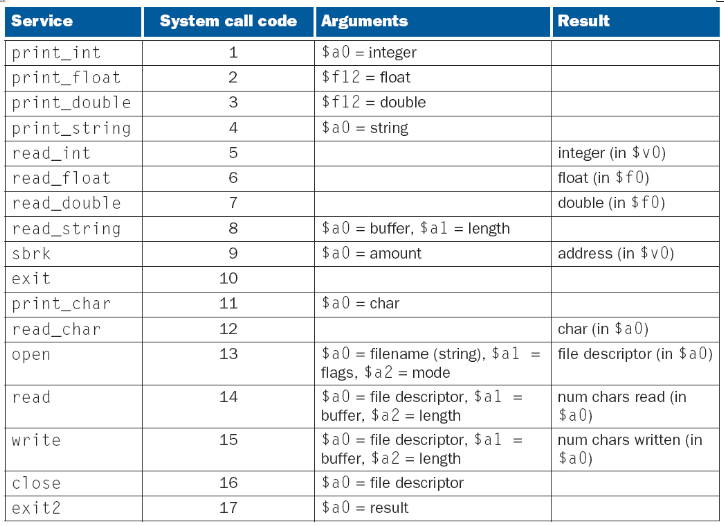
\includegraphics[width=100mm, scale=0.5]{tabella syscall.png}
\end{center}

\chapter{Datapath}
Il datapath è un insieme di unità di calcolo, come ad esempio
ALU, i registri e i moltiplicatori necessari per l'esecuzione delle istruzioni nella
CPU.
Il passaggio di due operando attraverso la ALU e la memorizzazione del risultato in un
nuovo registro viene detto ciclo di data path. Tale ciclo definisce ciò che è in grado
di fare una macchina: più veloce è questo ciclo, più veloce sarà la macchina.

\section{Realizzare un datapath}
\begin{itemize}
    \item Si stabilisce il set di istruzioni da implementare
    \item Si identificano i componenti del datapath (Alu, register file, ecc)
    \item Si stabilisce la metodologia di clocking
    \item Si assembla il datapath e si identificano i segnali di controllo
    \item Si analizza l'implementazione di ogni istruzione per determinare il setting
    dei segnali di controllo
    \item Si analizza l'implementazione di ogni istruzione per determinare il setting
    dei segnali di controllo
    \item Si assembla la logica di controllo
\end{itemize}

\section{Passi per l'esecuzione di una istruzione - Fetch Decode Execute}
\subsection*{Fetch} \begin{itemize}
    \item Legge l'istruzione dalla memoria e la salva in un registro dedicato
    (Instruction Register)
    \item L'indirizzo di memoria che indica l'istruzione da leggere si trova nel registro
    Program Counter (PC)
    \item Dopo la lettura dell'istruzione in PC, viene incrementato di 3 per indicare la
    prossima istruzione (usando l'ALU)
\end{itemize}
\subsection*{Decode}
Decodifica i vari campi dell'istruzione per decidere quali sono i passi necessari
per la sua esecuzione

\subsection*{Execute}
Esegue i passi necessari per eseguire l'istruzione

\section{Implementazione Fetch}
\begin{center}
    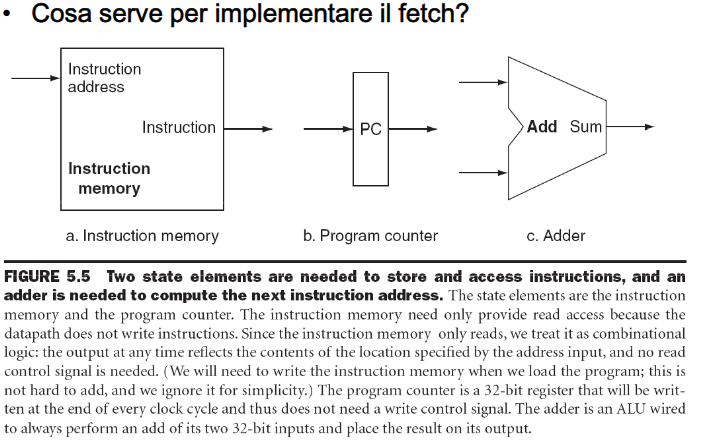
\includegraphics[width=100mm, scale=0.5]{Implementazione fetch.png}
\end{center}
\begin{center}
    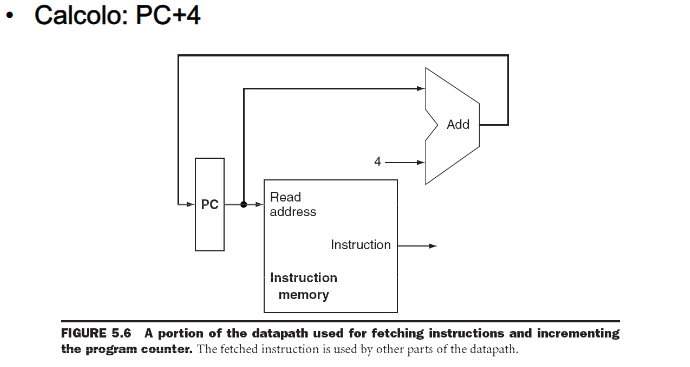
\includegraphics[width=100mm, scale=0.5]{Fetch PC+4.png}
\end{center}
Ciclo che ci permette in sostanza di caricare l'indirizzo di memoria iniziale e
poi incrementare il PC d 4 per passare all'istruzione successiva
\section*{Decode}
Il processore MIPS legge i vari campi dell'istruzione e identifica il tipo di istruzione
da eseguire (OPCODE e FUNC CODE se necessario)
\section*{Execute}
\section*{Clocking}
Nello schema è implicito il clock, ci sono 2 metodologie principali
\paragraph*{Singolo ciclo} \begin{itemize}
    \item Ciclo singolo di lunghezza fissa uguale al tempo necessario per eseguire l'istruzione
    più lunga
    \item Ogni istruzione viene eseguita in un ciclo di clock
    \item Svantaggi: spreco di tempo, perchè per far sì che tutte le istruzioni vengano eseguite in 
    un clock solo devo avere un clock più lento.
\end{itemize}

\paragraph*{Multi-ciclo} \begin{itemize}
    \item Ciclo di lunghezza fissa più corretto
    \item Ogni istruzione viene eseguita in più cicli di clock
    \item Istruzioni di tipo diverso - eseguite in un numero di cicli di clock diverso
    \item Maggiore ottimizzazione rispetto al singolo ciclo
    \item Più complesso perchè devo orchestrare (unità di controllo) la gestione dei clock
\end{itemize}

\section{Datapath multi-ciclo}
Servono dei registri aggiuntivi (oltre ai 32 che abbiamo già visto)
\begin{itemize}
    \item Memorizzano valori intermedi che vengono usati nel ciclo di clock successivo
    per continuare l'esecuzione della stessa istruzione
    \item Instruction Register - Tiene in memoria la copia dell'istruzione che sto utilizzando
    \item MDR - Memory Data Regiser - Copia dei dati da elaborare prelevati dalla memoria 
    \item A, B - registri tra register File e l'ingresso Alu - tengono in memoria i registri contenenti gli operando
    \item ALUout - l'output della ALU (dato che l'ALU è un circuito combinatorio non è in 
    grado di memorizzare un risultato)
\end{itemize}

\section{Dettaglio esecuzione istruzioni MIPS}
\begin{itemize}
    \item Fetch dell'istruzione e incremento PC
    \item Decode: decodifica dell'istruzione E lettura registri E calcolo
    dell'indirizzo per un eventuale branch
    \item Execute: eseguire le operazionmi relative a R\_type OPPURE calcolo di memoria
    OPPURE completa branch OPPURE completa kump
    \item Execute: completa R\_type OPPURE accesso alla memoria
    \item Execute: scrittura registro (solo per l'istruzione lw)
\end{itemize}

\section{Datapath: Automa per il controllo}
Un automa che ripete all'infinito la sua esecuzione, serve per controllare il datapath.
Spiega nel dettaglio il ciclo Fetch Decode Execute. 

\section{Riassumendo il Datapath}
\begin{center}
    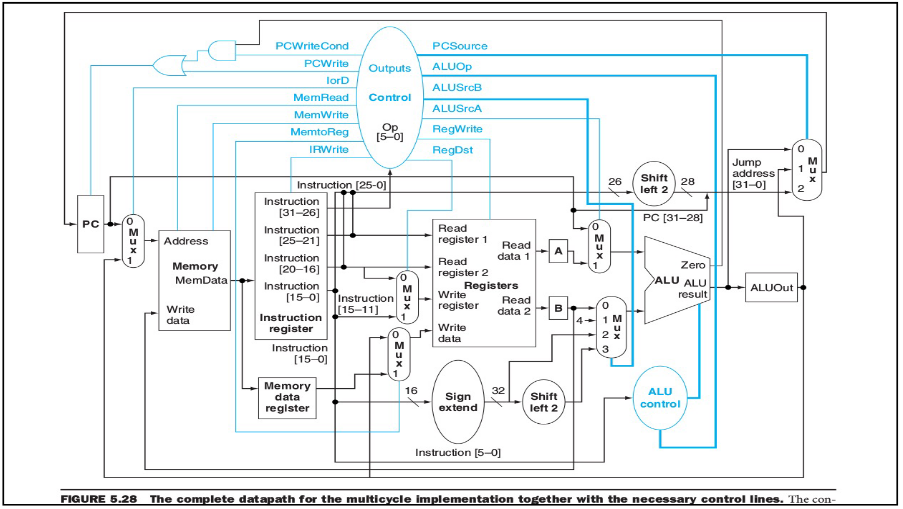
\includegraphics[width=100mm, scale=0.5]{Datapath.png}    
\end{center}
\paragraph*{Memoria} Contiene istruzioni e dati sulla base dell'indirizzo in input
restituisce in output l'istruzione o il dato letto.
\paragraph*{Register File} 32 registri che contengono i dati utilizzati nel corso
dell'esecuzione delle istruzioni, restituisce in output il contenuto dei due registri
letti (indicati dai due input - ReadRegister1 e ReadRegister2) e scrivere, se il segnale
di scrittura è attivo, il dato in input WriteData nel registro indicato dall'indirizzo
in input (WriteRegister).
\paragraph*{ALU} per tutte le istruzioni incrementa il PC (PC+4) e calcola il valore
di branch (che sarà usato solo nel caso di istruzioni di branch).
Inoltre:
\begin{itemize}
    \item Istruz R-Type: esegue operazioni aritmetico logiche su due operandi in funzione
    del "function code" indicato dai 6 bit meno significativi dell'istruzione
    \item Istr. accesso a memoria: calcola l'indirizzo di memoria cui accedere
    \item Istr. branch: confronta i due registri in input
\end{itemize}
\paragraph*{Sign Extended}: opera l'estensione di segno dai 16 bit in input ai 32 bit in output.
\paragraph*{Shift Left 2} opera uno shift a sinistra dei bit in input (con l'effetto di 
moltiplicare per 4 l'input)

\subsection{Funzioni dei registri}
\paragraph*{PC}: contiene i 32 bit che indicano l'indirizzi dell'istruzione da eseguire
\paragraph*{Instruction Register} Contiene i 32 bit che corrispondono alla codifica
dell'istruzione prelevata da memoria per l'esecuzione
\paragraph*{Memory Data Register} contiene il dato letto da memoria prima della sua scrittura
nel registro destinazione (e.g. nel caso di esecuzione di istruzione load)
\paragraph*{A e B} Contengono i valori letti dai registri del RegisterFile
\paragraph*{ALUOut} Contiene l'output della ALU
\subsection{Ruolo di ciascuno dei multiplexer}
\begin{center}
    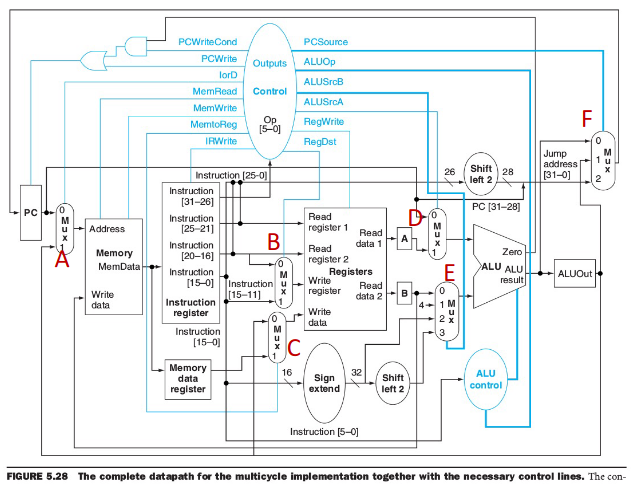
\includegraphics[width=100mm, scale=0.5]{Datapath Multiplexer.png}
\end{center}
\paragraph*{A} seleziona l'indirizzo di memoria a cui acedere tra:
\begin{itemize}
    \item PC (nel caos is voglia leggere un'istruzione)
    \item output della ALU (nel caso di esecuzione dell'istruzione "load")
\end{itemize}
\paragraph*{B} Seleziona il gruppo di bit dell'IR che indirca il registro in cui scrivere
i due tipi di istruzione I-Type (IT[20:16]) e R-type (IR[15:11])
\paragraph*{C}Seleziona la sorgente per il dato da scrivere in memoria tra:
\begin{itemize}
    \item ALUOut (per istruzioni R-type)
    \item MemoryDataRegister (per istruzioni load)
\end{itemize}
\paragraph*{D} Seleziona il primo operando dell'operazione aritmetico-logica eseguita
dalla ALU tra PC (per incrementeo +4) e registro A (per istruzioni R-type)
\paragraph*{E} Seleziona il secondo operando dell'operazione aritmetico-logica eseguita
dalla ALU
\begin{itemize}
    \item B (per istruzioni R-type)
    \item 4 (per aggiornamenti del PC)
    \item sign-extended IR[15:0] (per istruzioni di accesso a memoria - lw/sw)
    \item sign-extended 2-shifted (j)
\end{itemize}
\paragraph*{F} Seleziona il valore per l'aggiornamento del PC
\begin{itemize}
    \item output dell'ALU: PC + 4
    \item contenuto di ALUOut: 2 shifted 26-bit beq field
    \item jump target address (IR[25:0] shifted left 2 bits e concatenato con PC + 4)
\end{itemize}

\subsubsection{Segnali di controllo fetch, decode, execute}
L'attivazione dei segnali di controllo per un datapath multiciclo può essere descritta
da un \textbf{automa a stati finiti}.
\\ I segnali di controllo (next state per l'automa) sono definiti \textbf{in funzione dello stato
corrente e dell'Opcode}.
\\ \textbf{Per tutti i tipi di istruzioni}, nella fase di fetch (stato 0) sono impostati i
seguenti segnali:
\begin{itemize}
    \item IorD = 0 per selezionare PC come sorgente per l'indirizzo di memoria
    \item MemRead: per leggere un'istruzione da memoria
    \item IRWrite per scrivere l'istruzione letta nell'Instruction register
    \item ALUSrcA, ALUSrcB, ALUOp, PCWrite e PCSource sono impostati per calcolare
    PC + 4 e memorizzare il nuovo valore nel PC
\end{itemize}
\textbf{Per tutti i tipi di istruzioni}, nella fase di decode (stato 1) sono impostati
i segnali ALUSrca, ALUSrcB e ALUOp per calcolare il valore di branch
\\ Nella fase di execute sono impostati i segnali di controllo, \textbf{in funzione del tipo di
istruzione in esecuzione}.
\begin{itemize}
    \item Le istruzioni di \textbf{jump o branch}, dopo lo stato 1 richiedono un ciclo di clock per
    il loro completamento
    \item Le istruzioni di tipo R-type e le istruzioni di memorizzazione (store), richiedono
    due cicli di clock per l'esecuzione di una sequenza di due stati d'impostazione dei segnali
    \item Le istruzioni di lettura da memoria richiedono tre cicli di clock per l'esecuzione
    di una sequenza di tre stati d'impostazione dei segnali
\end{itemize}
\begin{center}
    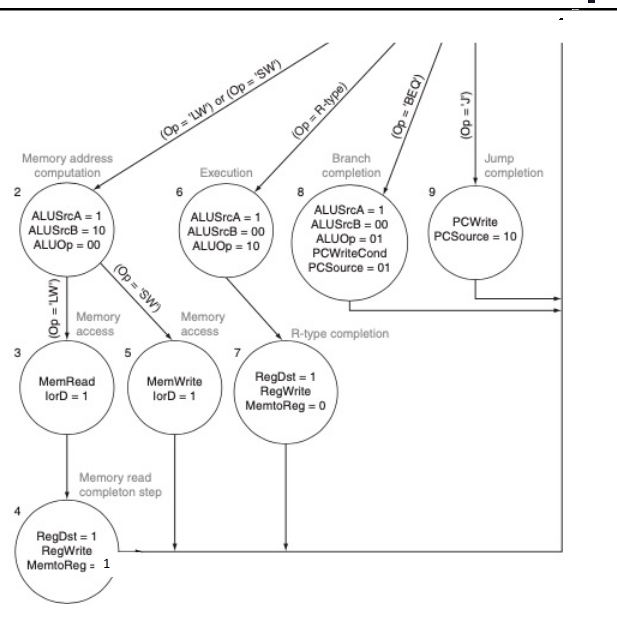
\includegraphics[width=100mm, scale=0.5]{Datapath automa.png}
\end{center}
% Fare esercizi con numero di cicli effettuati per eseguire istruzioni assembly

\section{Eccezioni}
Durante l'esecuzione delle istruzioni si possono verificare eventi inattesi: eccezioni
e/o interruzioni.
\paragraph*{Eccezione} Evento sincrono generato all'interno del processore e provocato
da problemi nell'esecuzioni di un'istruzione. Per esempio un overflow, una istruzione
no nvalida, errori, pagine non presenti in memoria, ecc.
\begin{itemize}
    \item Causate da eventi interno al processore
    \item Sincrone rispetto al programma in esecuzione
    \item La condizione di eccezione deve essere risolta da un gestore di eccezioni (es. handler)
    \item Se la condizione do eccezione è risolvibile il programma riprendere l'esecuzione, altrimenti
    il programma termina prima della sua fine.
\end{itemize}

\paragraph*{Interruzione} Evento asincrono che giunge dall'esterno del processore.
Di solito arriva da un'unità di I/O utilizzato per comunicare alla CPU il verificarsi
di certi eventi.
Esempi: la terminazione di un'operazione di I/O la cui esecuzioni era stat richiesta dalla
CPU.
\begin{itemize}
    \item Causate da eventi esterni al processore
    \item Asincrone rispetto al programma in esecuzione
    \item Sono gestite tra due istruzioni consecutive
    \item Si sospende l'esecuzione del programma utente, si gestisce l'interruzione e poi
    si riprende l'esecuzione del programma utente
\end{itemize}

\subsection{Gestione di eccezioni e interruzioni}
Il controllo del processore deve gestire gli eventi inattesi.
Tutti i processori eseguono i seguenti passi per gestire un eccezione/interruzione:
\begin{itemize}
    \item Interruzione dell'esecuzione del programma corrente
    \item Salvataggio parziale dello stato in esecuzione corrente (e.g. PC) - per
    riprendere eventualmente l'esecuzione del programma corrente se possibile
    \item Salto a una routine del sistema operativo (SO) per gestire l'eccezione/interruzione
    (tale routine è chiamata di solito handler o gestore delle eccezioni)
    \item Esecuzione della routine del SO
    \item Se possibile, ripristino dello stato di esecuzione del programma
    e continuazione dell'esecuzione del programma
\end{itemize}
\paragraph*{Come capire l'evento inatteso verificatosi?}
Due possibili soluzioni:
\begin{enumerate}
    \item Indirizzo fisso - Registro dedicato (e.g., Cause) - il controllo della CPU,
    prima di saltare all'handler del SO (a un indirizzo fisso), deve salvare in un registro
    interno un identificatore numerico del tipo di eccezione verificatosi.
    L'handler accederò al registro interno per determinare la causa dell'eccezione
    \item Interruzioni vettorizzate - esistono handler diversi per eccezioni/interruzioni differenti.
    il controllo della CPU sceglie l'handler corretto, saltando all'indirizzo corretto.
    A questo scopo, viene predisposto un vettore di indirizzi, uno per ogni tipo
    di eccezione/interruzione, da indirizzare tramite il codice numerico dell'eccezione/interruzione
\end{enumerate}
\paragraph*{MIPS} In MIPS viene adottata la prima soluzione, usando un registro, denominato
Cause, per memorizzare il motivo dell'eccezione. L'indirizzo dell'istruzione corrente che ha causato
l'eccezione viene salvato nel registro Exception Program Counter (EPC).

\subsection*{Esempio di gestione delle eccezioni in MIPS}
Passi da eseguire:
\begin{itemize}
    \item Individuare l'evento inatteso, la causa dell'eccezione e salvarla in un registro
    dedicato denominato Cause
    \item interrompere l'esecuzione corrente
    \item Salvare l'indirizzo dell'istruzione corrente nel EPC (EPC = PC - 4)
    \item Saltare a un gestore delle eccezioni del SO che si trova a un indirizzo
    fisso per gestire l'eccezione
\end{itemize}
\paragraph*{Osservazioni}
\begin{itemize}
    \item Il MIPS non salva nessun altro registro oltre al PC
    \item è compito della routine salvare altre porzioni dello stato corrente del programma
    se necessario
    \item Esistono CPU dove questo salvataggio avviene prima di saltare alla routine (es approcci CISC)
\end{itemize}

\paragraph*{Necessario aggiungere 2 stati} 
\begin{itemize}
    \item Devono salvare in EPC il valore PC - 4
    \item Salvare nel registro Cause la causa dell'eccezione (0 o 1 in questo caso perchè
    consideriamo 2 esempi di eccezioni)
    \item Salvare in PC l'indirizzo del gestore delle eccezioni
\end{itemize}
\subsection*{Pratica MIPS}
Per tutti i tipi di eccezione avviene
\begin{itemize}
    \item Salvataggio dell'indirizzo dell'istruzione che ha causato l'eccezione (in EPC)
    \item Cambiamento del normale flusso di esecuzione di un programma: aggiornamento di PC
    con il valore 0x80000180 che corrisponde all'indirizzo dello spazio kernel text in cui
    ha inizio la procedura di gestore delle eccezioni - exception handler.
\end{itemize}
\begin{center}
    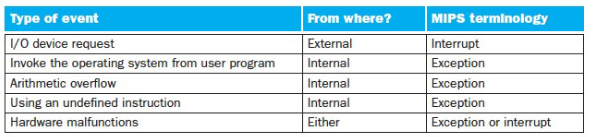
\includegraphics[width=100mm, scale=0.5]{Eccezioni e interruzioni.png}
\end{center}
\paragraph*{Il registro Cause e possibile cause di eccezione}
\begin{center}
    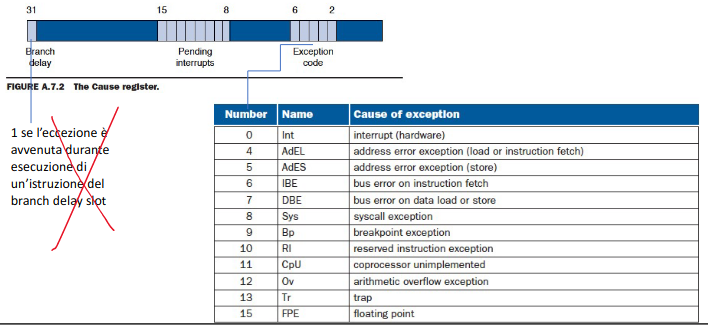
\includegraphics[width=100mm, scale=0.5]{Possibili cause di eccezione.png}
\end{center}

\subsubsection*{Exception Handler}
\'E la porzione di codice assembly che contiene il codice che gestisce le eccezioni
e si trova alla locazione fissa 0x80000180 in area ktext riservata al sistema operativo.
Quando si presenta un eccezione viene caricato nel PC l'indirizzo dell'Handler, così che
venga eseguito il codice che si occupa di capire di che eccezione si tratta.
\\ Dal momento che viene eseguito dopo l'interruzione di un programma utente in un punto
qualsiasi, è tenuto a \textbf{preservare TUTTI i registri macchina}. Ad esso sono riservati
i due registri \textbf \$k01, \$k02 che può utilizzare senza doverne preservare i contenuti.
Al termine del trattamento dell'eccezione, l'exception handler ritorna il controllo al programma
interrotto (istruzione eret).
MIPS rileva e tratta eccezioni PRIMA del completamento dell'esecuzione della istruzione corrente.
\begin{itemize}
    \item Se è una interruzione, dopo la sua gestione, l'esecuzione del programma deve
    riprendere dall'istruzione corrente (salvata nel registro EPC)
    \item si si tratta di una eccezione ed è possibile proseguire l'esecuzione deve riprendere
    dall'istruzione successiva (EPC+4).
\end{itemize}

%Fare esercizi gestione eccezioni (exception handler)

%Caricare gestore eccezioni e programma che genera overflow

\chapter{Gestione Input-Output}
Con I/O definiamo l'insieme di architetture e dispositivi per il trasferimento di informazioni da 
e verso l'elaboratore. Si tratta di dispositivi eterogenei per
\begin{itemize}
    \item Velocità di trasferimento
    \item Latenze
    \item Sincronizzazione
    \item Modalità di interazione (sia con l'uomo che con la macchina)
\end{itemize}
\section{Bus di Sistema}
Esistono vari tipi di bus nei computer di oggi. In questo corso tratteremo il bus di sistema
che collega la CPU con la memoria e con le periferiche.
Il bus di sistema è composto da:
\begin{itemize}
    \item Bus di dati: le linee per trasferire dati e istruzioni da/verso dispositivi
    \item Bus di controllo: trasporta informazioni per la definizione delle operazioni
    da compiere per la sincronizzazione fra i dispositivi
    \item Bus degli indirizzi: la CPU trasmette gli indirizzi di memoria o di perificheria che
    identificano i dati da leggere/scrivere dalla memoria/periferiche
\end{itemize}
Tutte le unità dell'elaboratore sono connesse al bus
\paragraph*{Vantaggi} Elevata flessibilità, semplicità, basso costo
\paragraph*{Svantaggi} Gestione complessa del canale condiviso

\section{Periferiche}
Sono dispositivi per I/O di informazioni collegati alla CPU tramite il bus di sistema e/o interfacce,
le interfacce sono standardizzate per la comunicazione e hanno una componente hardware (e.g. il controller
della periferica) e una componente software (e.g. driver).
La struttura di un'interfaccia contiene reistri di dati (oppure buffer) e ha associato registri di stato.

\subsection*{Periferiche mappate in memoria}
Una parte della memoria riservata al sistema viene usata per la comunicazione con le periferiche.
Ogni periferica ha uno spazio dedicato nella memoria e viene assegnato un identificatore unico alla stessa
(es. indirizzo unico).
\\ I registri dell'interfaccia della periferica sono mappati in memoria, ma sono riservati, per questo non sono accessibili da
un programma utente, per potervi accedere è necessario passare dal SO.
\\ L'accesso alla periferica è simile all'accesso alla memoria (e.g. lw, sw) dal punto di vista della CPU.
Non tute le architetture degli elaboratori usano questa soluzione.
\subsection*{Un selettore generale per mappare dispositivi in memoria}
\begin{center}
    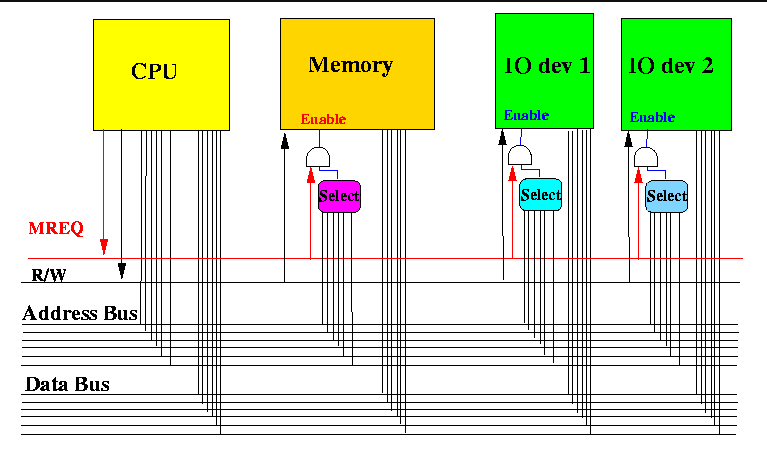
\includegraphics[width=100mm, scale=0.5]{selettore per mappare periferiche.png}
\end{center}
\subsection*{Registri di interfaccia della periferica}
Il \textbf{registro di stato della periferica} rappresenta lo stato della stessa e viene letto dalla CPU. Un esempio di stato è 
"periferica pronta per ricevere dati, dati richiesti disponibili per il trasferimento.
Il \textbf{registro dei dati della periferica} rappresenta i dati di input o di output in base al tipo della stessa.
\subsection{Passi di I/O}
\begin{enumerate}
    \item CPU interroga lo stato della periferica
    \item La periferica restituisce il suo stato
    \item Se la periferica è pronta per trasmettere/ricevere dati, la CPU richiede il trasferimento dei dati
    \item La CPU invia o riceve i dati
\end{enumerate}
\subsection{Tecniche di gestione I/O}
\begin{itemize}
    \item I/O gestito da programma (Programmed I/O)
    \item I/O guidato da interrupt (Interrupt Driven I/O)
    \item Accesso Diretto alla Memoria (Direct Memory Access - DMA)
\end{itemize}
Per valutare le prestazioni del trasferimento dati è necessario ricorrere a delle misure che permettono
di valutare l'efficienza della gestione delle operazioni di I/O.
\begin{itemize}
    \item Banda passante - rappresenta la quantità dei dati che si può trasferire per unità di tmepo;
    rappresenta una misura di flusso
    \item Latenza - rappresenta il tempo che interoccre tra l'istante in cui una periferica è pronta
    per il trasferimento e l'istante in cui il dato viene trasferito, è una misura di tmepo
\end{itemize}

\subsection*{I/O Gestito da programma}
In questa casistica è il programma a gestire l'I/O e la periferica ha un ruolo passivo.
La CPU si occupa sia del controllo sia del trasferimento dati, predisponendo il controllore
della periferica all'esecuzione dell'I/O. 
\\ La CPU si ferma e interroga il registro di stato della periferica in attesa che sia pronta (e.g.
ready bit assume un determinato valore).
\paragraph*{Vantaggio} Risposta veloce al ready bit
\paragraph*{Svantaggio} la CPU resta bloccata in stato di busy waiting
\begin{center}
    \includegraphics*[width=100mm, scale=0.5]{IO gestito da programma.png}
\end{center}
\paragraph*{Prestazioni I/O gestito da programma}
\begin{itemize}
    \item Banda passante alta perchè la CPU trasferisce subito il dato (molti dati per l'unità
    di tempo) e la gestione della periferica richiede poche istruzioni
    \item Latenza minima in quanto la CPU noterà subito lo stato della periferica (tempo massimo:
    un ciclo intero di busy waiting)
\end{itemize}
Esempio: se si trasferiscono più dati si ha un ciclo interno per il trasferimento di ogni byte 
e un ciclo esterno per il trasferimento di tutti i byte.

\subsection*{I/O gestito da interrupt}
L'Interrupt è un evento asincrono che genera l'interruzione del normale funzionamento del processore.
\begin{itemize}
    \item La periferica segnala alla CPU di aver bisogno di attenzione mediante un segnale sul bus di controllo,
    tale segnale è una segnale \textbf{interrupt request}
    \item Quando il processore se ne accorge (in una fase di fetch) informa al periferica con un segnale 
    interrupt acknowledge. 
    \item La CPU interrompe l'esecuzione del programma corrente (salvando il contesto dell'esecuzione del programma per poter 
    riprendere la sua esecuzione) ed esegue la procedura di risposta all'interrupt.
    \item Terminata l'esecuzione della procedura di interrupt, la CPU riprendere l'esecuzione del programma
    interrotto, infine il programma utente continua la sua esecuzione.
\end{itemize}

\paragraph*{Vantaggio} La CPU non fa più busy waiting come per I/O gestito da programma
\paragraph*{Svantaggio} La CPU deve comunque gestire le operazioni di trasferimento
Per evitare l'intervento della CPU nella fase di trasferimento dati è stato introdotto il protocollo di trasferimento
DMA - Direct Memory Access.

\paragraph*{Prestazioni}
\begin{itemize}
    \item Banda passante: minor banda passante in quanto il trasferimento di ogni dato necessità di più tempo
    \item Latenza: maggior latenza per la maggior quantità di operazioni da eseguire 
\end{itemize}

\subsection*{DMA - accesso diretto alla memoria}
Usato quando si trasferiscono velocemente grandi quantità di dati.
Con \textbf{DMA} la periferica diventa autonoma negli accessi alla memoria dato che è essa a
gestire i trasferimenti, non è più la CPU a intervenire. Necessità di 2 registri in più
per ogni periferica oltre al registro di stato e registro dei dati.
\begin{itemize}
    \item Un registro che indichi l'indirizzo di memoria da/dove trasferire i dati
    \item Un registro che indichi la quantità dei dati da trasferire
\end{itemize}
Anche questi 2 registri aggiuntivi sono \textbf{mappati in memoria}.
\\ Alla fine del trasferimento la periferica invia un interrupt alla CPU per segnalare il completamento 
del trasferimento.
\paragraph*{Prestazioni}
\begin{itemize}
    \item Banda passante: massima perchè la CPU non deve eseguire nessuna istruzione
    \item Latenza: minima dato che nessuna istruzione è eseguita dalla CPU
\end{itemize}

%Gestione I/O con interruzione e DMA 1:14:00

\chapter{Gerarchie di memoria e cache}
L'ideale sarebe avere a disposizione una quantità illimitata di memoria e contemporaneamente
veloce, ma ciò non è possibile, dato che le memorie veloci costano molto di più a parità
di bit rispetto alle memorie lente.
Solitamente una memoria più capiente è più lenta, mentre una più veloce è meno capiente.
\begin{center}
    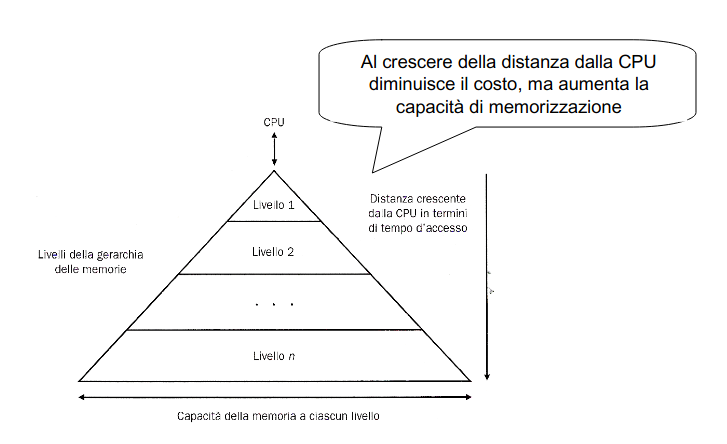
\includegraphics[width=100mm, scale=0.5]{Gerarchie memorie.png}
\end{center}
\paragraph*{CPU} La memoria interna alla CPU è costituita dai registri ed è caratterizzata
da alta velocità e limitate dimensioni.
\paragraph*{Memoria centrale} La memoria centrale è caratterizzata da dimensioni molto
maggiori della memoria interna alla CPU, ma con tempi di accesso più elevati. accessibile
direttamente tramite indirizzi. 
\\ Nei sistemi attuali è presente un livello intermedio in termini di capienza e velocità,
tra CPU e memoria centrale, esso è \textbf{la memoria cache}.
\paragraph*{Memorie secondarie} Sono ad alta capacità, con bassi costi e non volatili.

\section{Principio di località}
Un programma in un certo istante di tempo, accede soltanto a una porzione relativamente
piccola del suo spazio di indirizzamento e questa è la base del comportamento dei programmi
in un calcolatore.
\paragraph*{Definizione} "Durante l'esecuzione di una data istruzione presente in memoria, 
con molta probabilità le successive istruzioni saranno ubicate nelle vicinanze
 di quella in corso.
Nell'arco di esecuzione di un programma si tende a fare riferimenti continui 
alle stesse istruzioni."
\\ Fonte Wikipedia 
\\ Esistono due tipi di località:
\begin{itemize}
    \item Temporale: quando si fa riferimento a un elemento c'è tendenza a fare
    riferimento allo stesso elemento dopo poco tempo
    \item Spaziale: quando si fa riferimento a un elemento c'è la tendenza a fare riferimenti
    poco dopo ad altri elementi che hanno l'indirizzo vicino ad esso
\end{itemize}
\paragraph*{Importante}I programmi NON vedono la gerarchia ma referenziano i dati come Se
fossero sempre in memoria centrale.
Il principio di località viene sfruttato strutturando la memoria in modo gerarchico.
\begin{itemize}
    \item Velocità - Più è veloce, più è vicina al processore, più è costosa
    \item Dimensione - Più è grande, più è lontana dal processore, meno è costosa
\end{itemize}
Un livello di memoria più vicino al processore contiene un sottoinsieme di dati memorizzati in ogni livello sottostante
e tutti i dati si trovano nel livello più basso.

\section{Definizioni}
\begin{itemize}
    \item \textbf{Blocco/linea} - La più piccola quantità di informazione che può essere presente/assente in una gerarchia
    di memoria
    \item \textbf{Hit (successo nell'accesso)} - L'informazione richiesta dal processore si trova in uno dei 
    blocchi nel livello superiore della memoria
    \item \textbf{Miss (fallimento nell'accesso)} - Il dato non è presente nel livello immediatamente superiore
    di memoria e occore accedere al livello più distante
    \item \textbf{Hit rate (frequenza di hit)} - Frazione degli accessi alla memoria nei quali l'informazione
    richiesta è stata trovata nel livello superiore di memoria
    \item \textbf{Miss rate (frequenza di miss)} - Frazione degli accessi alla memoria nei quali l'informazione
    richiesta NON è stata trovata nel livello superiore di memoria (1 - HitRate)
    \item \textbf{Tempo di hit} - Tempo di accesso al livello superiore della memoria
    \\ Comprende anche il tempo necessario a stabilire se il tempo di accesso si risolva in un successo 
    in un fallimento
    \item \textbf{Tempo di miss} - Il tempo necessario a sostituire un blocco del livello superiore con un nuovo 
    blocco dal livello inferiore della gerarchia, e trasferire i dati di questo blocco al processore
    \item \textbf{Frequenza di hit} = $\frac{\mbox{Accessi risolti con successo}}{\mbox{Numero totale di accessi}}$
    \item \textbf{Frequenza di miss} = $\frac{\mbox{Accessi risolti senza successo}}{\mbox{Numero totale di accessi}}$
\end{itemize}

\paragraph*{Remind} Una gerarchia di memoria può essere composta da più livelli, ma i dati venogno trasferiti solo
tra due livelli vicini.

\section{Cache}
La Cache è il livello della memoria gerarchia che si trova tra il processore e la memoria principale.
Proviene dal termine francese cachè, che significa nascosto. La memoria cache e il suo utilizzo sono generalmente
trasparenti al programmatore (quindi nascosta).
L'algoritmo per la gestione della cache, l'algoritmo di caching, si basa sui principi di località spaziale e temporale.
\begin{itemize}
    \item Mantiene i dati richiesti recentemente "vicino" alla CPU (località temporale)
    \item Muove blocchi contigui di memoria che contendono il dato richiesto (località spaziale)
\end{itemize}

\subsection{Tipi di cache}
\subsection*{Direct Mapped}
A ciascun blocco della memoria corrisponde una specifica locazione nella cache, viene direttamente assegnato
uno specifico blocco.
Associa una sola locazione della cache a ogni parola della memoria definendo una corrispondenza tra l'indirizzo
in memoria della parola e la locazione nella cache.
\begin{center}
    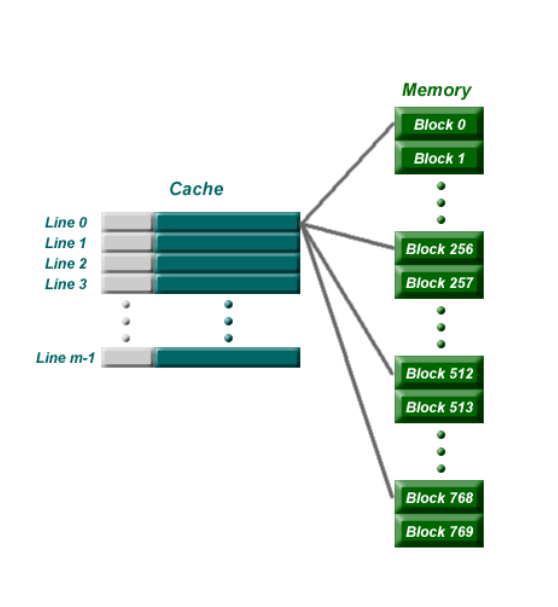
\includegraphics[width=60mm, scale=0.5]{Direct mapped cache.png}
    \includegraphics[width=60mm, scale=0.5]{Direct mapped cache conflict.png}
\end{center}
Nella prima figura viene illustrato il funzionamento delle direct mapped cache, a ciascun
blocco di cache possono appartenere diversi blocchi di memoria.
Nella seconda figura notiamo che se un programma utilizza 2 indirizzi diversi si verifica
che lo stesso programma ha associati 2 indirizzi diversi, problema di associazione molti a uno.

\subsection*{Fully associative}
Una cache completamente associativa ci permette di memorizzare i dati in qualsasi blocco inutilizzato della cache,
anzichè forzare l'assegnazione di uno specifico blocco di memoria come nella direct mapped. Si risolve così la problematica
del conflitto. In questo caso la corrispondenza è 1 a 1.
\\ Il problema è che è molto costosa perchè l'indirizzo viene unicamente riservato a un elemento, quindi la cache occupa
più spazio rispetto al direct mapped. Inoltre per cercare un blocco nella cache è necessario cercarlo in tutte le linee
della cache. La ricerca sequenziale è troppo lenta e la ricerca in parallelo è molto costosa.
\begin{center}
    \includegraphics[width=100mm, scale=0.5]{Fully associative.png}
\end{center}

\subsection*{Set Associative Mapping}
Ibrido tra Direct Mapped e Fully Associative.
Un indirizzo di memoria viene mappato su un gruppo della cache detto Set. Si ragiona quindi su sottoinsiemi,
non direttamente su indirizzo.
\begin{center}
    \includegraphics[width=100mm, scale=0.5]{Set associative cache.png}
\end{center}
Ciascun blocco della memoria ha a disposizione un numero fisso ($>=2$) di locazioni cache.
 
%END------------------------------------------------------------------------

\end{document}